% vim: set tw=78 tabstop=4 shiftwidth=4 aw ai:
\documentclass{beamer}

\usepackage[utf8x]{inputenc}		% diacritice
\usepackage[romanian]{babel}
\usepackage{color}			% highlight
\usepackage{alltt}			% highlight
\usepackage{minted}

% highlight; comment this out in case you don't input code source files
\usepackage{code/highlight}		% highlight

\usepackage{hyperref}			% folosiți \url{http://...}
					% sau \href{http://...}{Nume Link}
\usepackage{verbatim}

\usepackage{subcaption}

\def\code#1{\texttt{#1}}

\setlength{\leftmargini}{.5pt}

\mode<presentation>
{ \usetheme{Berlin} }

% Încărcăm simbolurilor Unicode românești în titlu și primele pagini
\PreloadUnicodePage{200}

% Arătăm numărul frame-ului
\newcommand{\frameofframes}{/}
\newcommand{\setframeofframes}[1]{\renewcommand{\frameofframes}{#1}}

\setframeofframes{of}
\makeatletter
\setbeamertemplate{footline}
  {%
    \begin{beamercolorbox}[colsep=1.5pt]{upper separation line foot}
    \end{beamercolorbox}
    \begin{beamercolorbox}[ht=2.5ex,dp=1.125ex,%
      leftskip=.3cm,rightskip=.3cm plus1fil]{author in head/foot}%
      \leavevmode{\usebeamerfont{author in head/foot}\insertshortauthor}%
      \hfill%
      {\usebeamerfont{institute in head/foot}\usebeamercolor[fg]{institute in head/foot}\insertshortinstitute}%
    \end{beamercolorbox}%
    \begin{beamercolorbox}[ht=2.5ex,dp=1.125ex,%
      leftskip=.3cm,rightskip=.3cm plus1fil]{title in head/foot}%
      {\usebeamerfont{title in head/foot}\insertshorttitle}%
      \hfill%
      {\usebeamerfont{frame number}\usebeamercolor[fg]{frame number}\insertframenumber~\frameofframes~\inserttotalframenumber}
    \end{beamercolorbox}%
    \begin{beamercolorbox}[colsep=1.5pt]{lower separation line foot}
    \end{beamercolorbox}
  }
\makeatother

\setbeamertemplate{navigation symbols}{}%remove navigation symbols
\setbeamertemplate{caption}[numbered]

\title[Eliminarea recursivității în programele Java]{Eliminarea recursivității în programele Java}
\subtitle{Sesiunea de licență -- septembrie 2017}
\institute{Facultatea de Automatică și Calculatoare,\\
	Universitatea POLITEHNICA București}
\author[Andrei Silviu Dragnea]{Andrei Silviu Dragnea\\
	Coordonator: Prof. dr. ing. Lorina Negreanu}
\date{11 septembrie 2017}

\begin{document}

% Slide-urile cu mai multe părți sunt marcate cu textul (cont.)
\setbeamertemplate{frametitle continuation}[from second]

% Arătăm numărul frame-ului
%\setbeamertemplate{footline}[frame number]

\frame{\titlepage}

%\frame{\tableofcontents}

% NB: Secțiunile nu sunt marcate vizual, ci doar apar în cuprins
\section{Context}

% Titlul unui frame se specifică fie în acolade, imediat după \begin{frame},
% fie folosind \frametitle
\begin{frame}{Recursivitatea}
%    \begin{columns}[T]
%        \begin{column}{\textwidth}
%            \begin{figure}
%                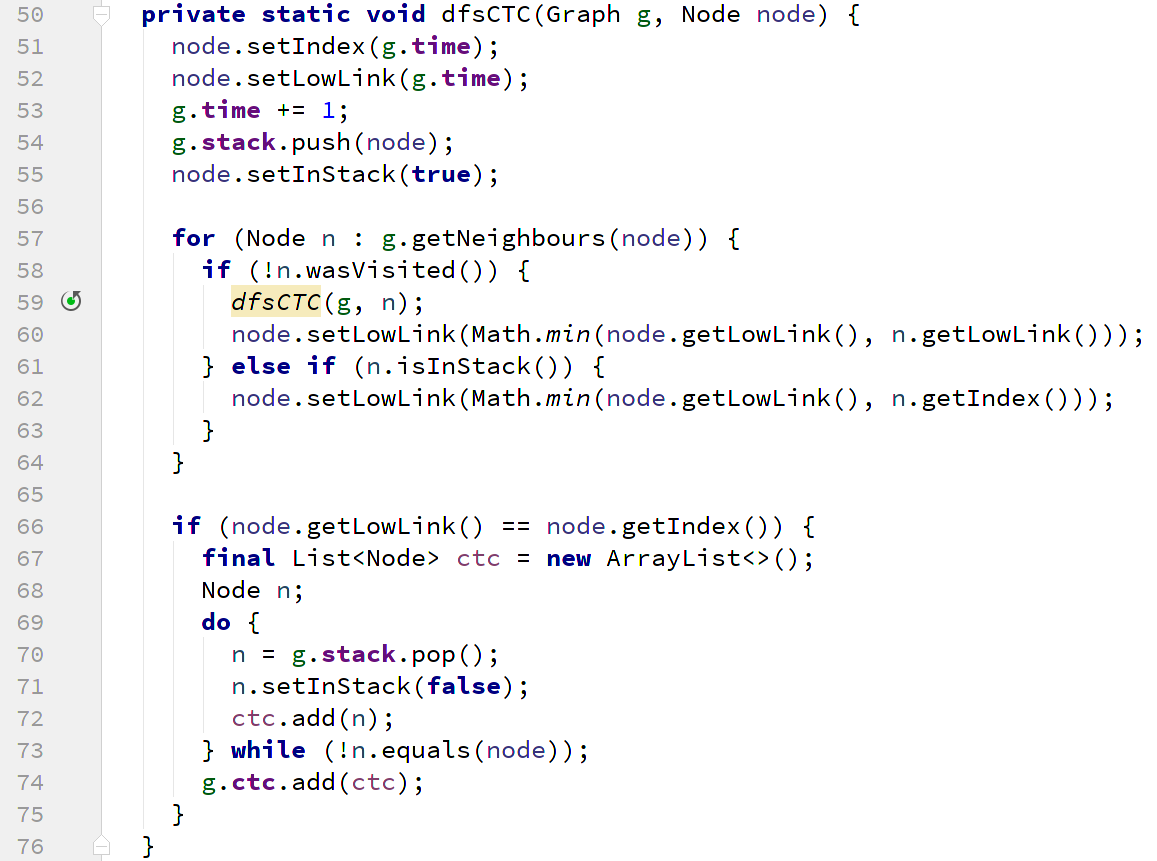
\includegraphics[height=6cm]{img/highlight}
%            \end{figure}
%        \end{column}
%    \end{columns}
    \begin{itemize}
        \item Recursivitatea este expresivă, dar uneori ineficientă
        \item În Java, compilatorul nu elimină niciun fel de recursivitate
        \item Programatorul alege care funcții trebuie transformate
        \item Funcționalitatea implementată ca un plugin pentru Intellij IDEA
    \end{itemize}
\end{frame}

\begin{frame}{Particularități ale recursivității în Java}
    \begin{itemize}
        \item Dacă metoda recursivă este statică sau privată, atunci apelul se rezolvă la compilare
        \item În caz contrar, apelul trebuie să fie făcut direct sau prin \code{this}
    \end{itemize}
\end{frame}

\begin{frame}{Algoritmul de eliminare a recursivității}
    \begin{itemize}
        \item Încapsularea instrucțiunilor în blocuri
        \item Expandarea buclelor \code{foreach}
        \item Extragerea apelurilor recursive în instrucțiuni separate
        \item Generarea clasei corespunzătoare unei înregistrări de activare
        \item Includerea corpului metodei în codul auxiliar
        \item Tratarea variabilelor locale
        \item Generarea grafului fluxului de control
        \item Eliminarea blocurilor inaccesibile
        \item Eliminarea blocurilor triviale
        \item Reducerea grafului de control
        \item Înlocuirea instrucțiunii return
    \end{itemize}
\end{frame}

\section{Implementare}

\begin{frame}{Încapsularea instrucțiunilor în blocuri}
    \begin{figure}[htb]
        \makebox[\linewidth][c]{%
        \begin{subfigure}[b]{.6\linewidth}
            \centering
            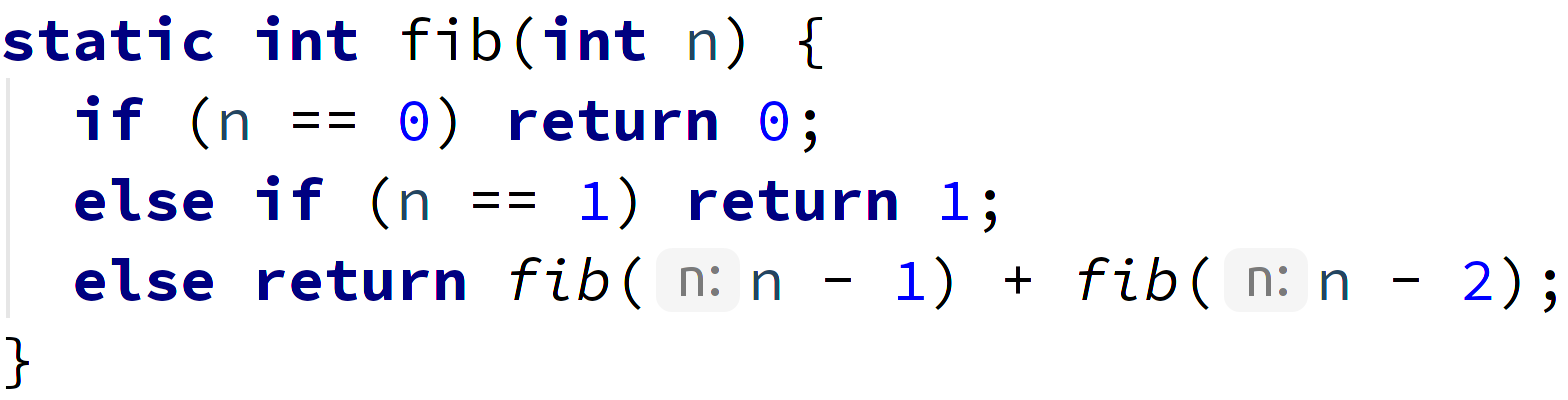
\includegraphics[height=0.6in]{../../../theses/diploma/src/img/replace-single-statements-with-block-statements-before-white.png}
            \caption{Înainte}
        \end{subfigure}%
        \begin{subfigure}[b]{.6\linewidth}
            \centering
            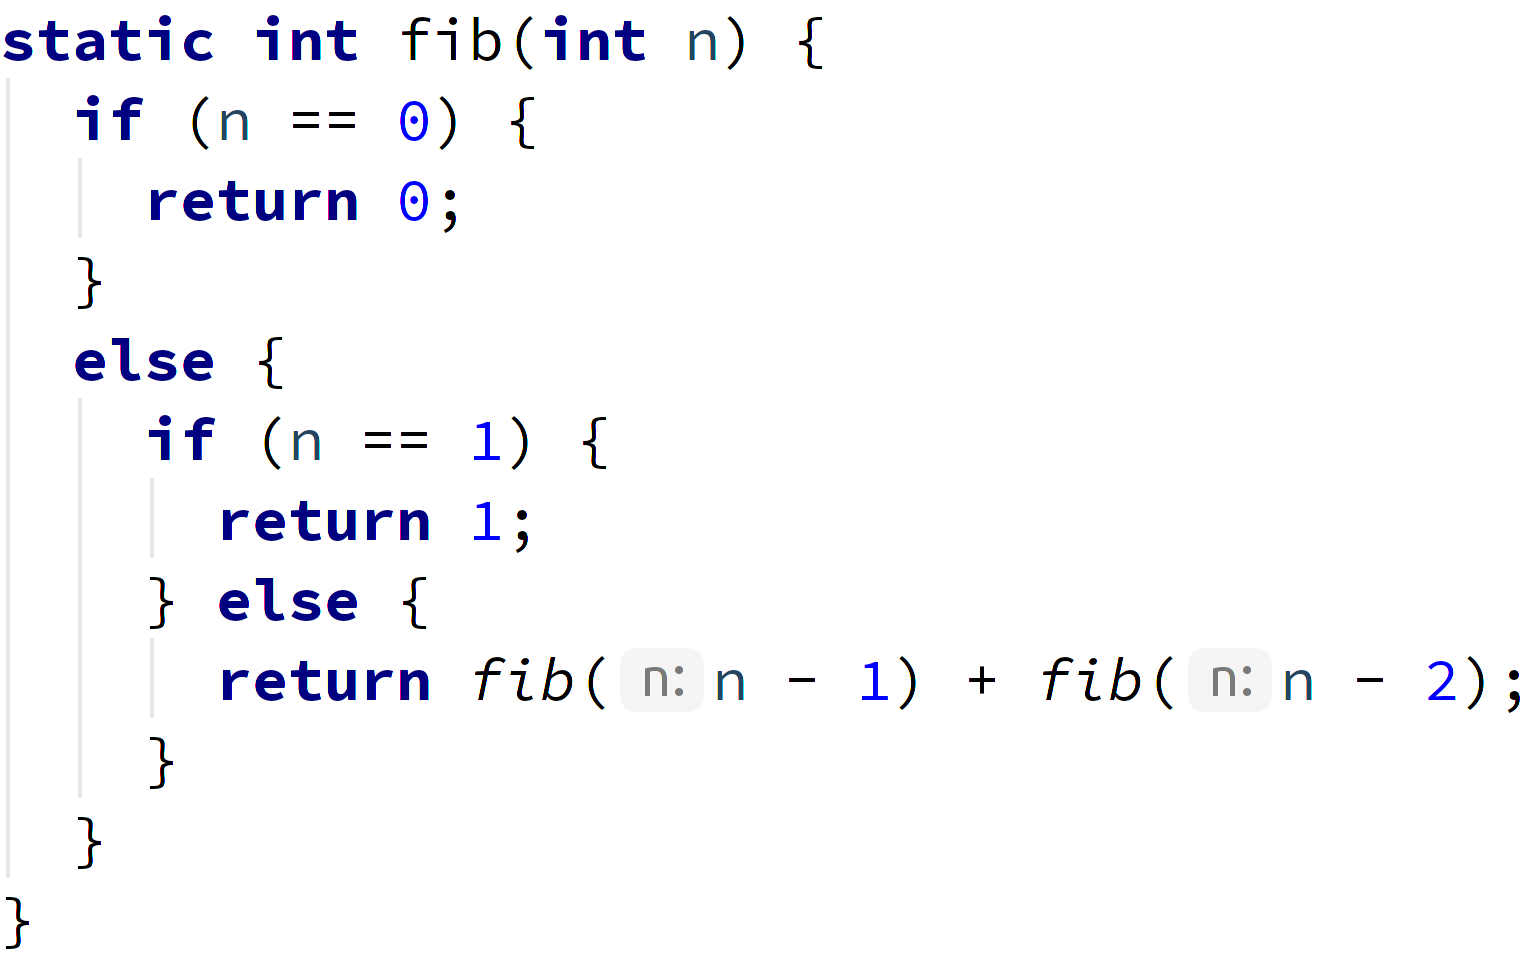
\includegraphics[height=1.44in]{../../../theses/diploma/src/img/replace-single-statements-with-block-statements-after-white.png}
            \caption{După}
        \end{subfigure}%
        }\\
%        \caption{Încapsularea instrucțiunilor în blocuri}
    \end{figure}
\end{frame}

\begin{frame}{Expandarea buclelor \code{foreach}}
    \begin{itemize}
        \item Expandarea \code{foreach} bazat pe iterator
        \begin{figure}[htb]
            \makebox[\linewidth][c]{%
            \begin{subfigure}[b]{.55\linewidth}
                \centering
                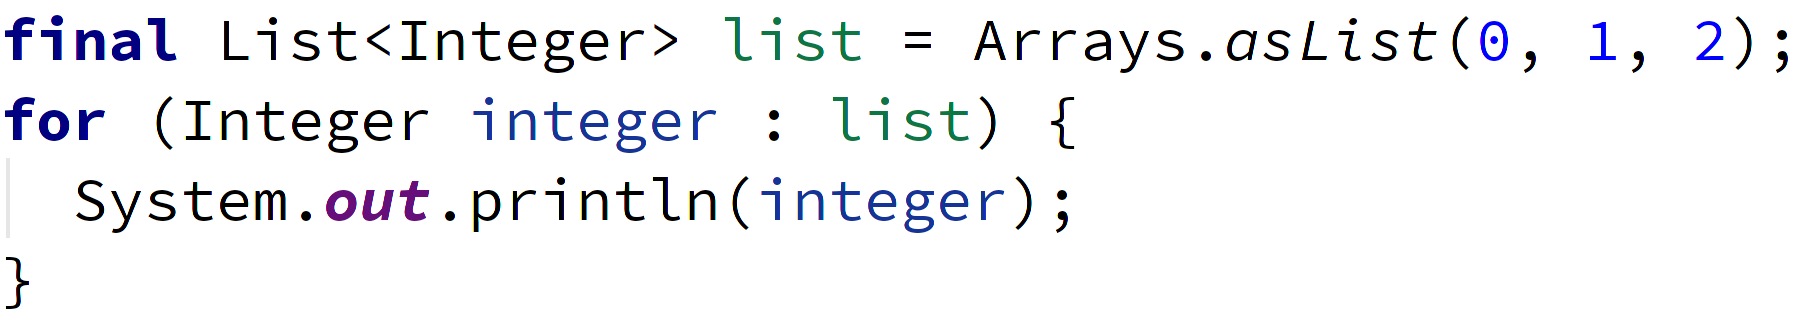
\includegraphics[height=0.4in]{../../../theses/diploma/src/img/foreach-to-iterator-for-before-white.png}
                \caption{Înainte}
            \end{subfigure}%
            \begin{subfigure}[b]{.55\linewidth}
                \centering
                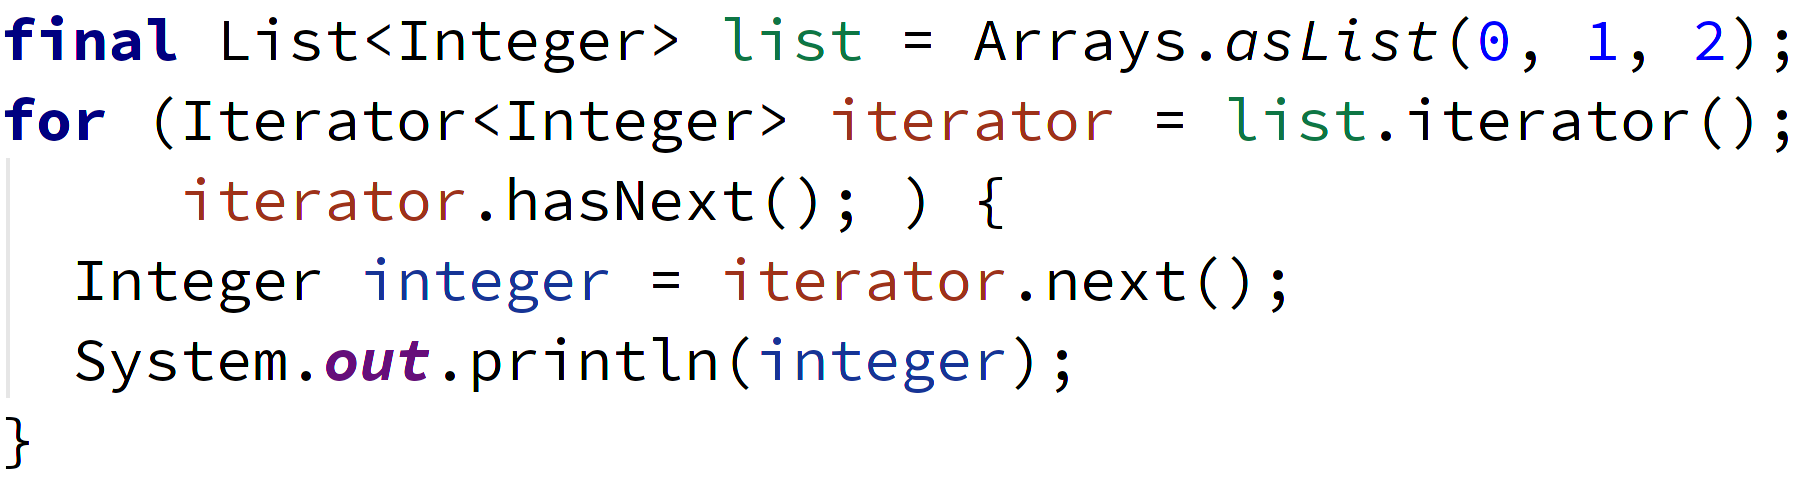
\includegraphics[height=0.6in]{../../../theses/diploma/src/img/foreach-to-iterator-for-after-white.png}
                \caption{După}
            \end{subfigure}%
            }\\
        \end{figure}

        \item Expandarea \code{foreach} bazat pe array
        \begin{figure}[htb]
            \makebox[\linewidth][c]{%
            \begin{subfigure}[b]{.55\linewidth}
                \centering
                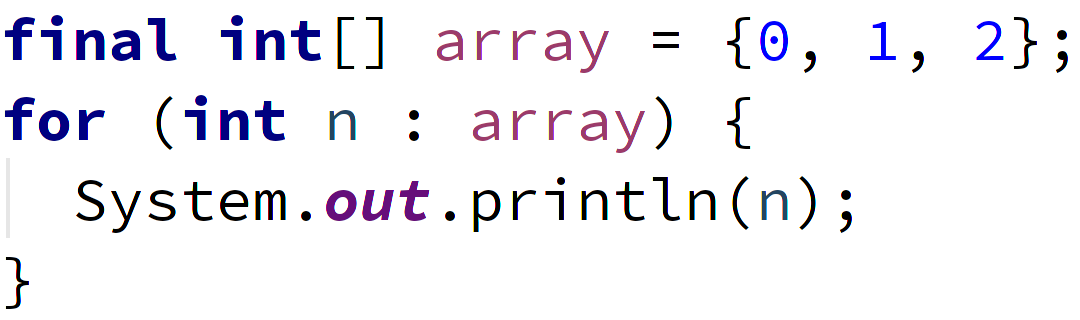
\includegraphics[height=0.4in]{../../../theses/diploma/src/img/foreach-to-indexed-for-before-white.png}
                \caption{Înainte}
            \end{subfigure}%
            \begin{subfigure}[b]{.55\linewidth}
                \centering
                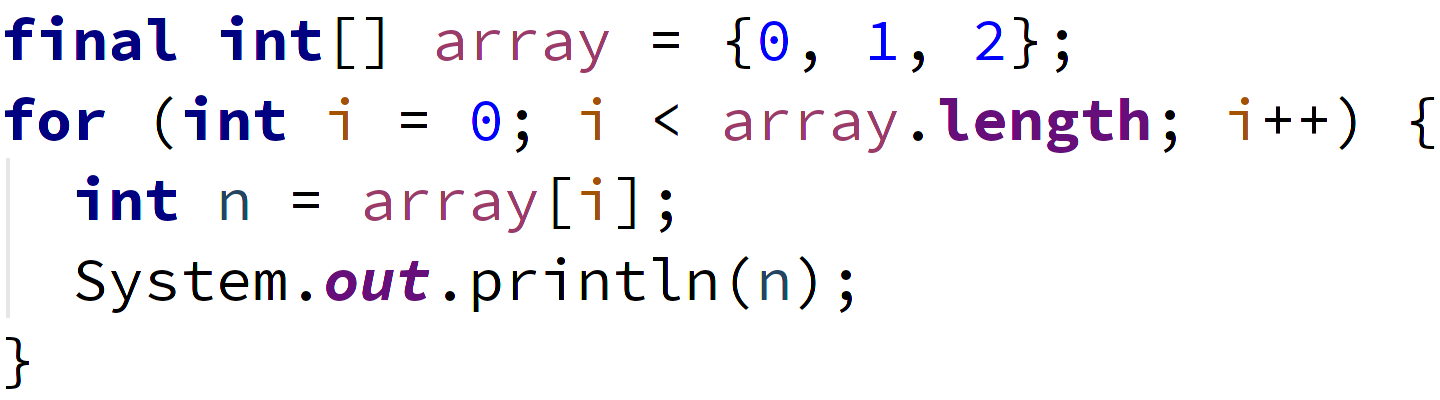
\includegraphics[height=0.5in]{../../../theses/diploma/src/img/foreach-to-indexed-for-after-white.png}
                \caption{După}
            \end{subfigure}%
            }\\
            % captions devin bullets
        \end{figure}
    \end{itemize}
\end{frame}

\begin{frame}{Extragerea apelurilor recursive în instrucțiuni separate}
    \begin{figure}[htb]
        \makebox[\linewidth][c]{%
        \begin{subfigure}[b]{.5\textwidth}
            \centering
            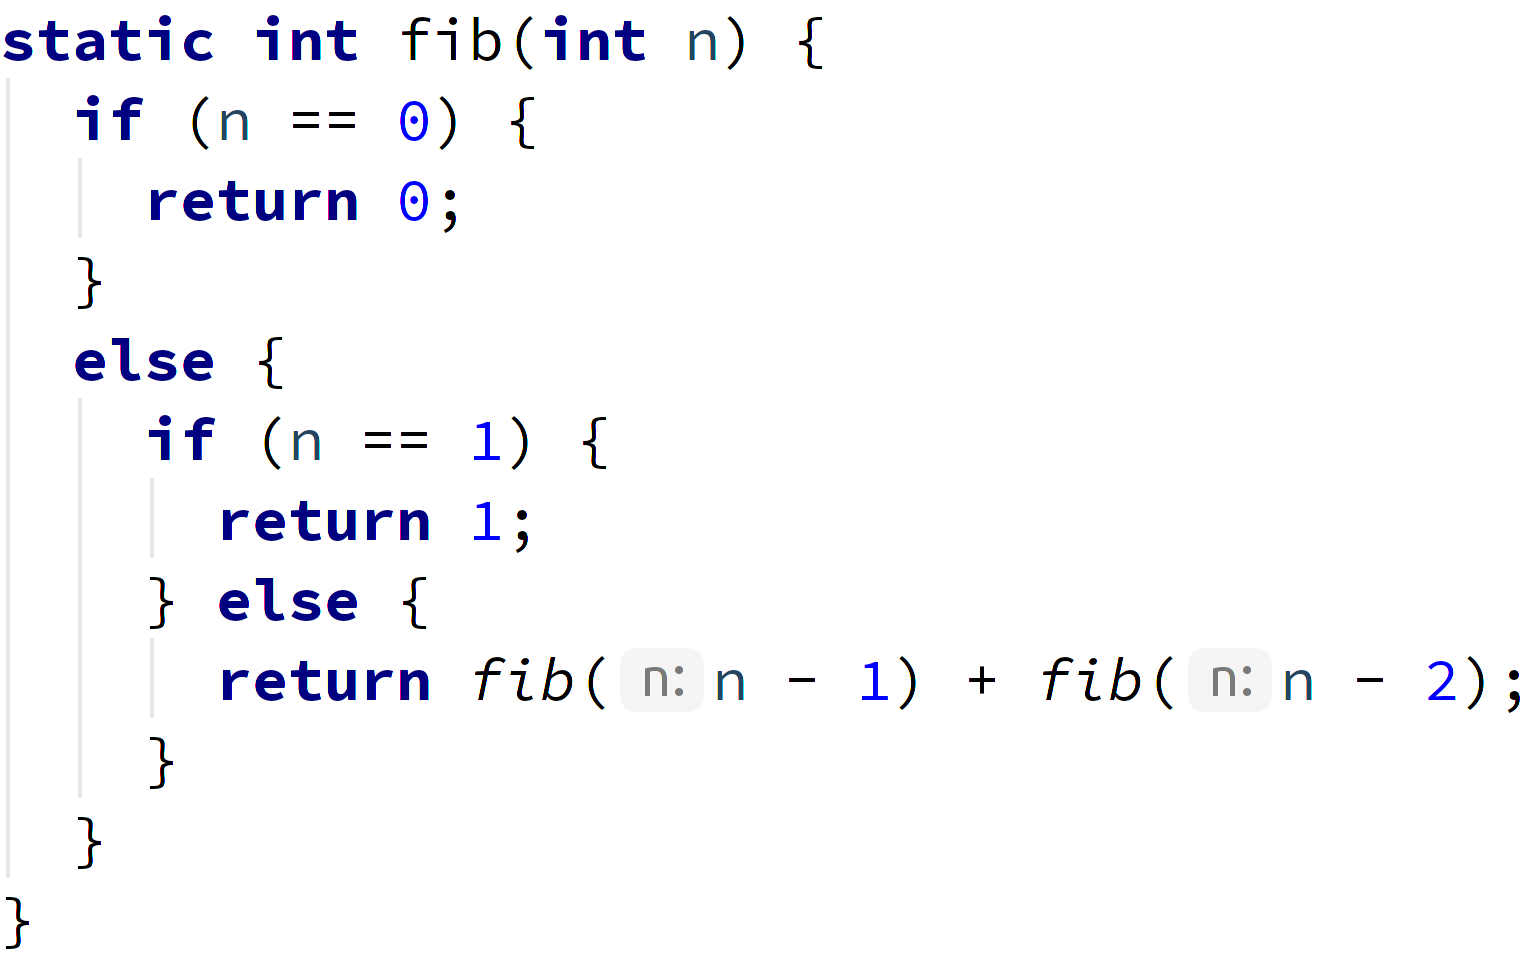
\includegraphics[height=1.44in]{../../../theses/diploma/src/img/replace-single-statements-with-block-statements-after-white.png}
            \caption{Înainte}
        \end{subfigure}%
        \begin{subfigure}[b]{.5\textwidth}
            \centering
            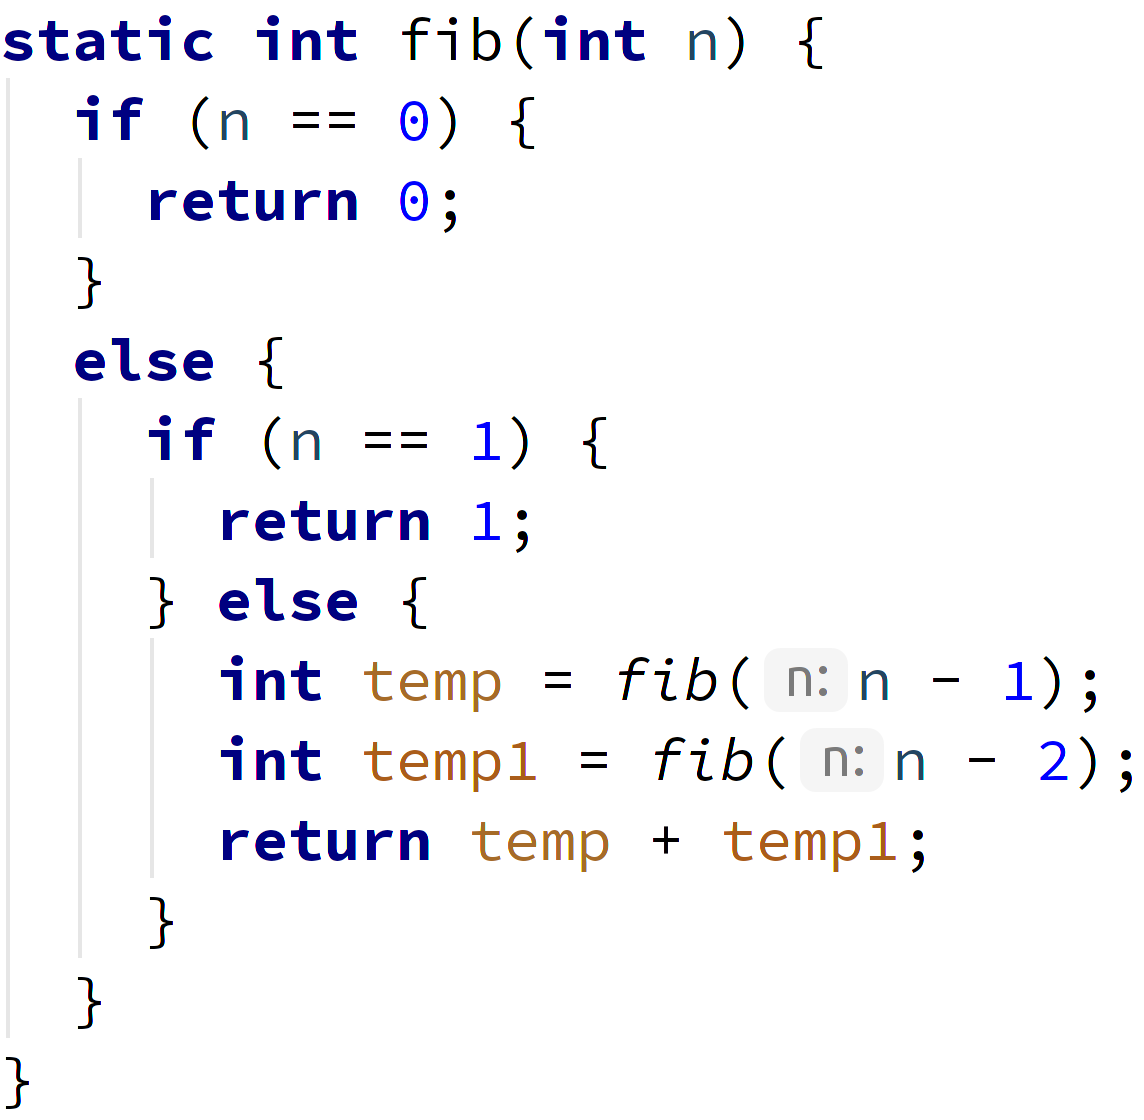
\includegraphics[height=1.68in]{../../../theses/diploma/src/img/extract-after-white.png}
            \caption{După}
        \end{subfigure}%
        }\\
%        \caption{Extragerea apelurilor recursive în instrucțiuni separate}
    \end{figure}
\end{frame}

\begin{frame}{Generarea clasei corespunzătoare unei înregistrări de activare}
    \begin{itemize}
        \item Colectarea parametrilor formali ai metodei și a declarațiilor de variabile locale
        \item Generarea unei clase statice ale cărei câmpuri corespund variabilelor locale
        \item Generarea câmpului \code{block}, care indică blocul din graful fluxului de control care trebuie executat
        la revenirea din apelul recursiv
    \end{itemize}
%    \begin{figure}[htb]
%        \makebox[\linewidth][c]{%
%        \begin{subfigure}[b]{.6\textwidth}
%            \centering
%            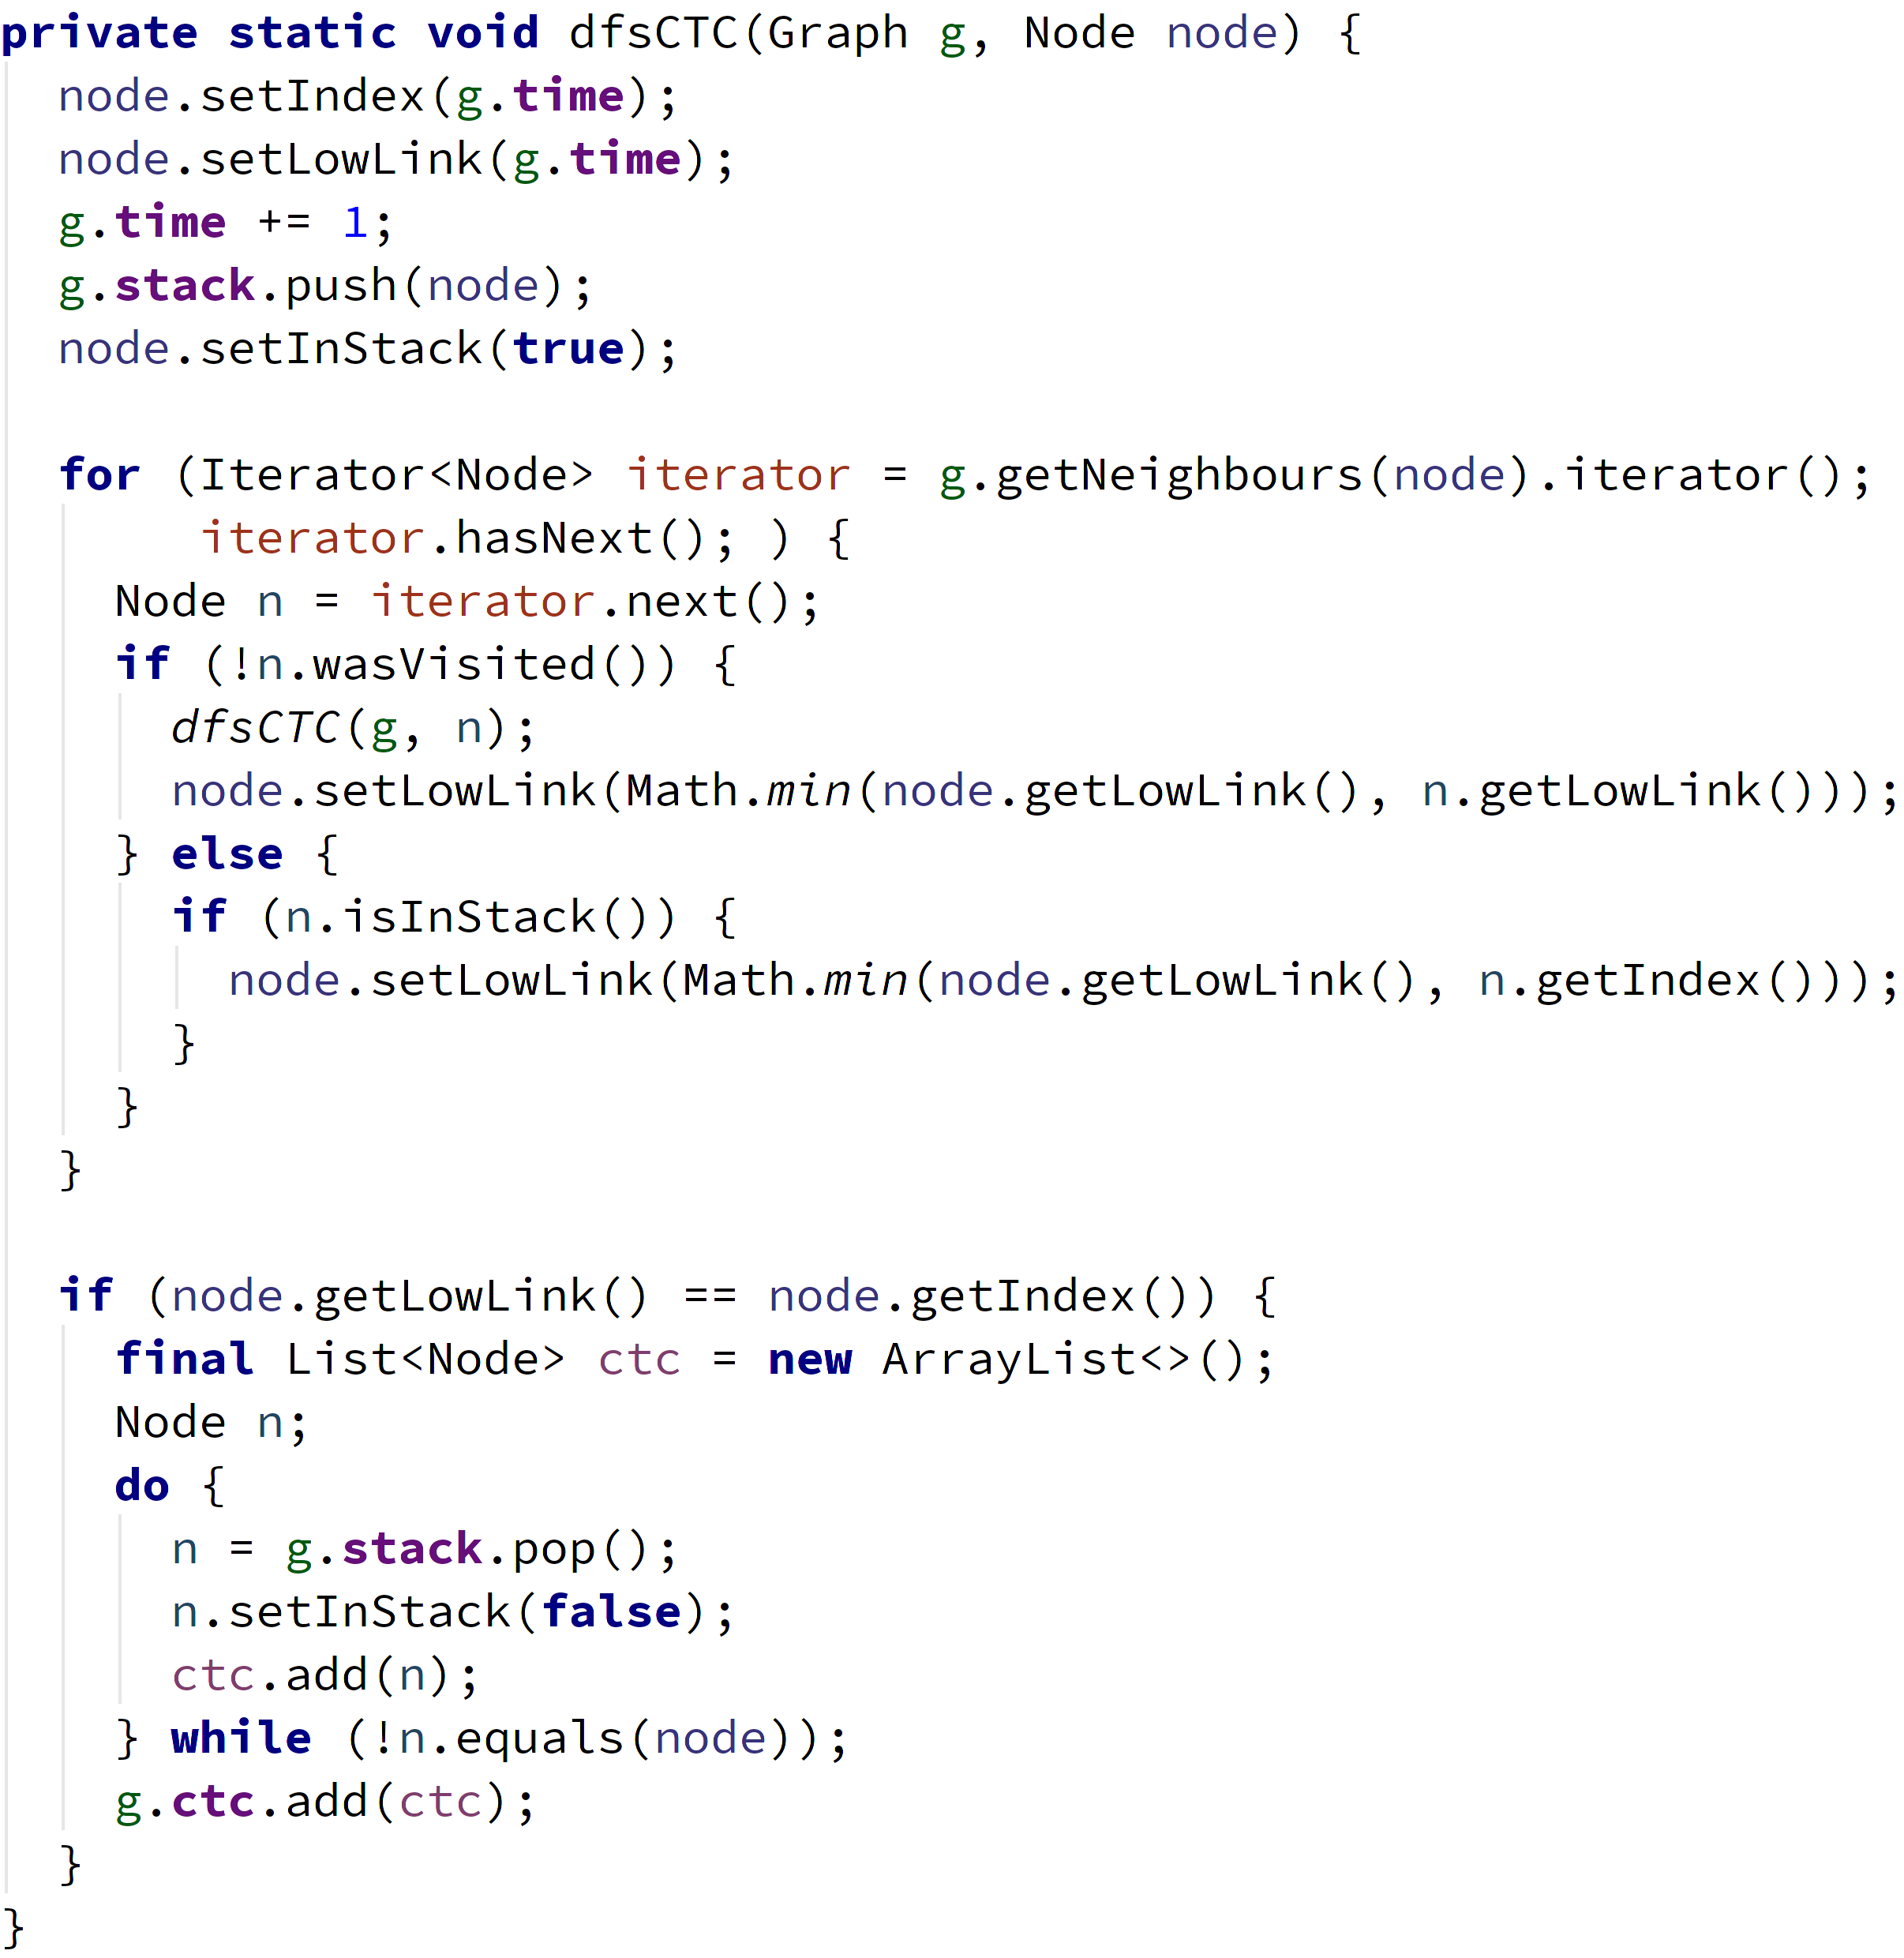
\includegraphics[height=1.75in]{../../../theses/diploma/src/img/add-frame-class-before-white-31.png}
%            \caption{Înainte}
%        \end{subfigure}%
%        \begin{subfigure}[b]{.6\textwidth}
%            \centering
%            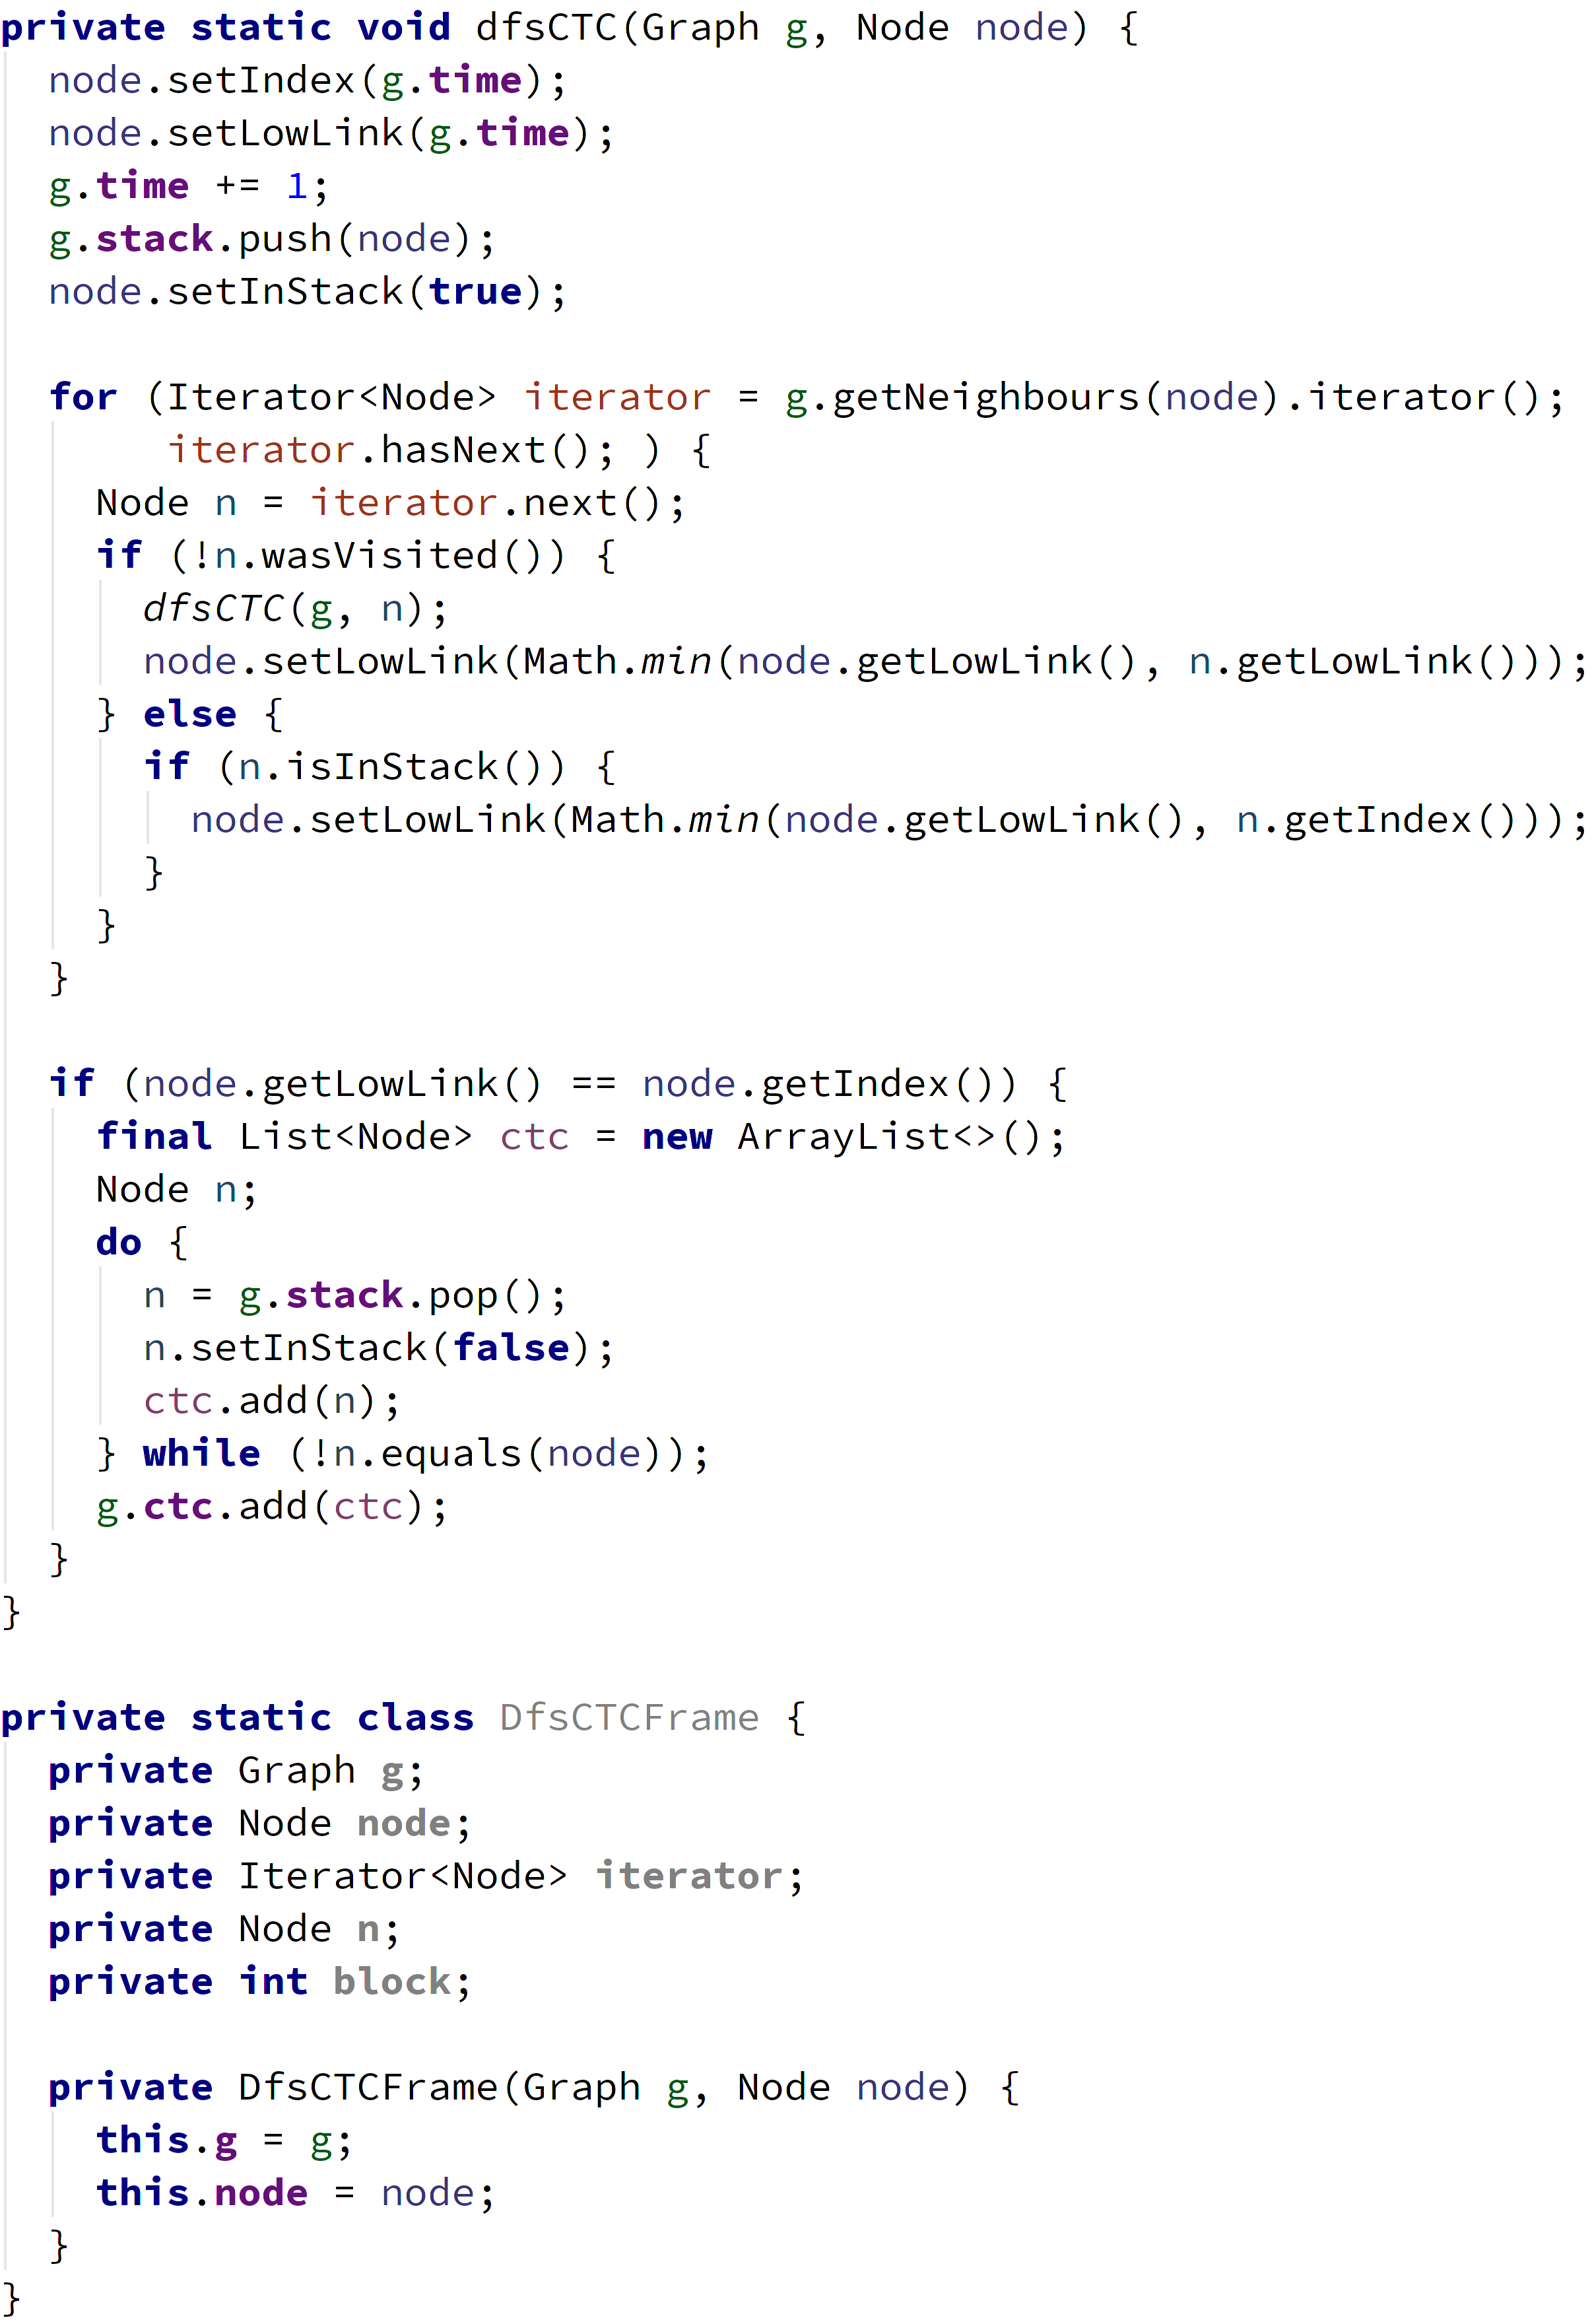
\includegraphics[height=2.484in]{../../../theses/diploma/src/img/add-frame-class-after-white-44.png}
%            \caption{După}
%        \end{subfigure}%
%        }\\
%        \caption{Generarea clasei cadru de stivă}
%    \end{figure}
\end{frame}

\begin{frame}{Includerea codului metodei în codul auxiliar}
%    \begin{figure}[htb]
%        \makebox[\linewidth][c]{%
%        \begin{subfigure}[b]{.5\textwidth}
%            \centering
%            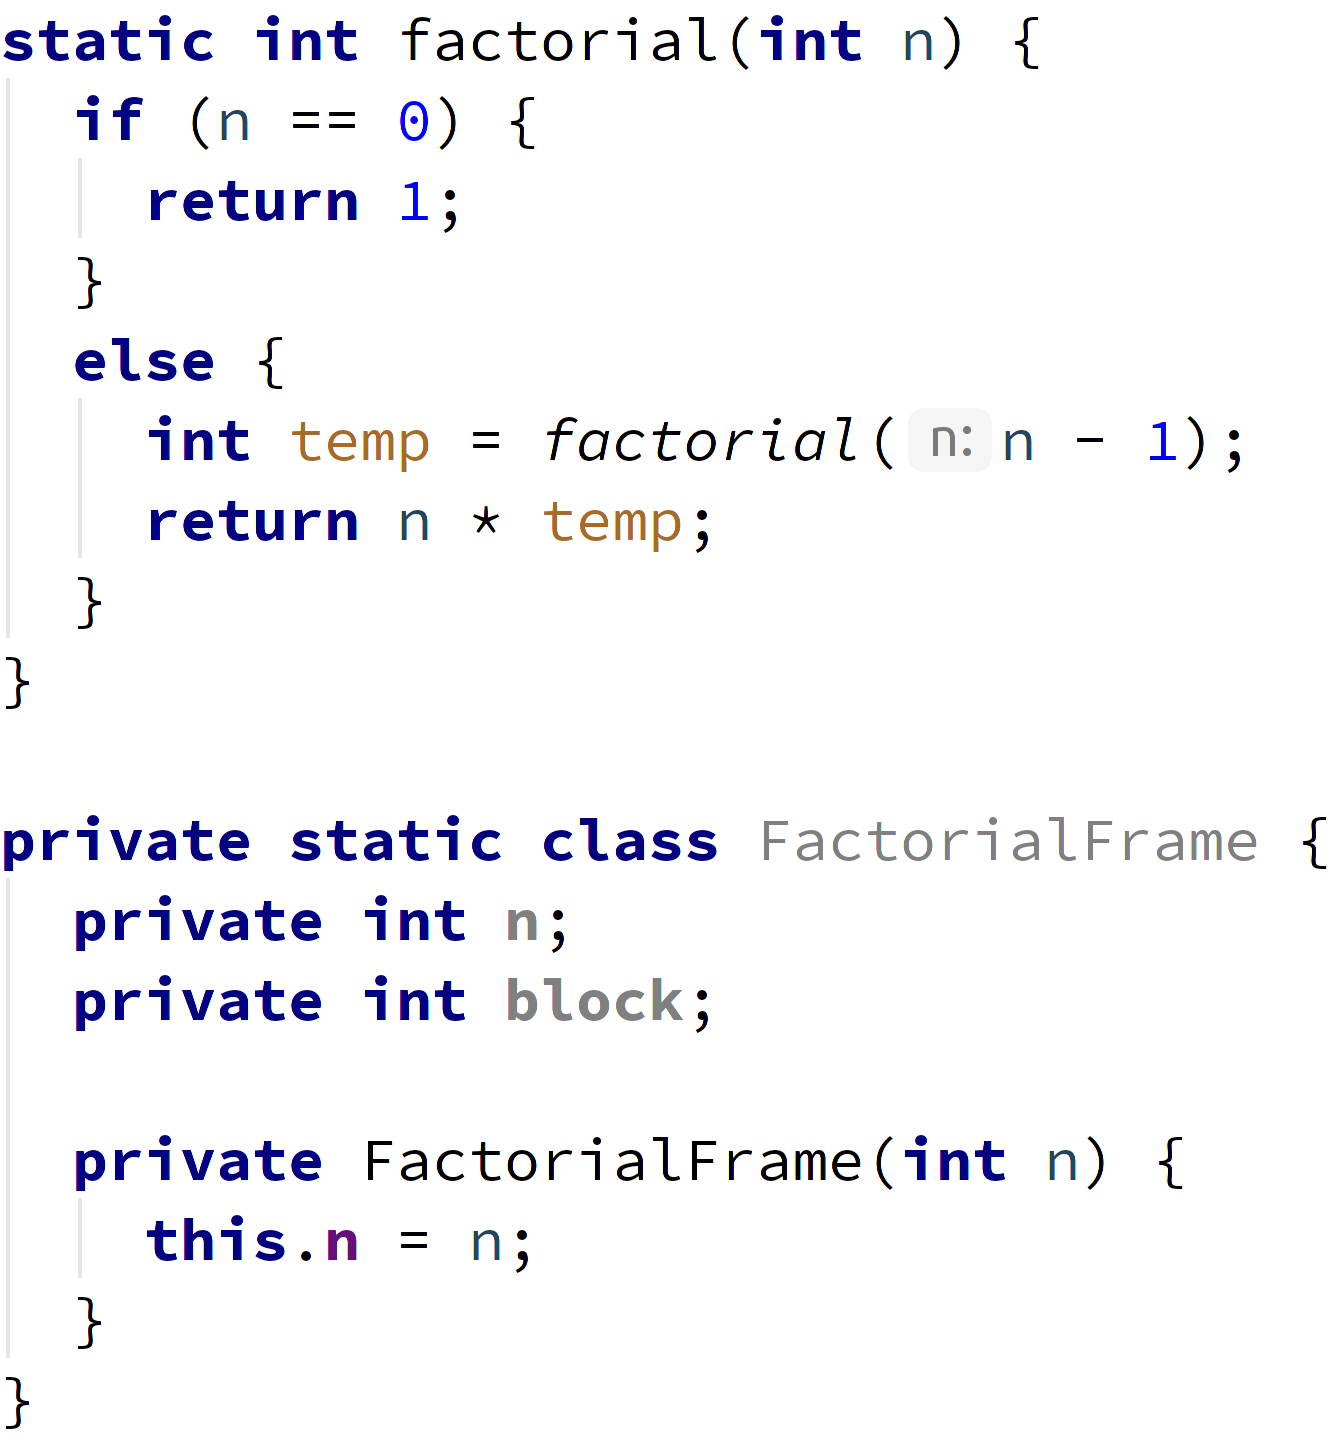
\includegraphics[height=1.7in]{../../../theses/diploma/src/img/incorporate-before-white-18.png}
%            \caption{Înainte}
%        \end{subfigure}%
%        \begin{subfigure}[b]{.5\textwidth}
%            \centering
%            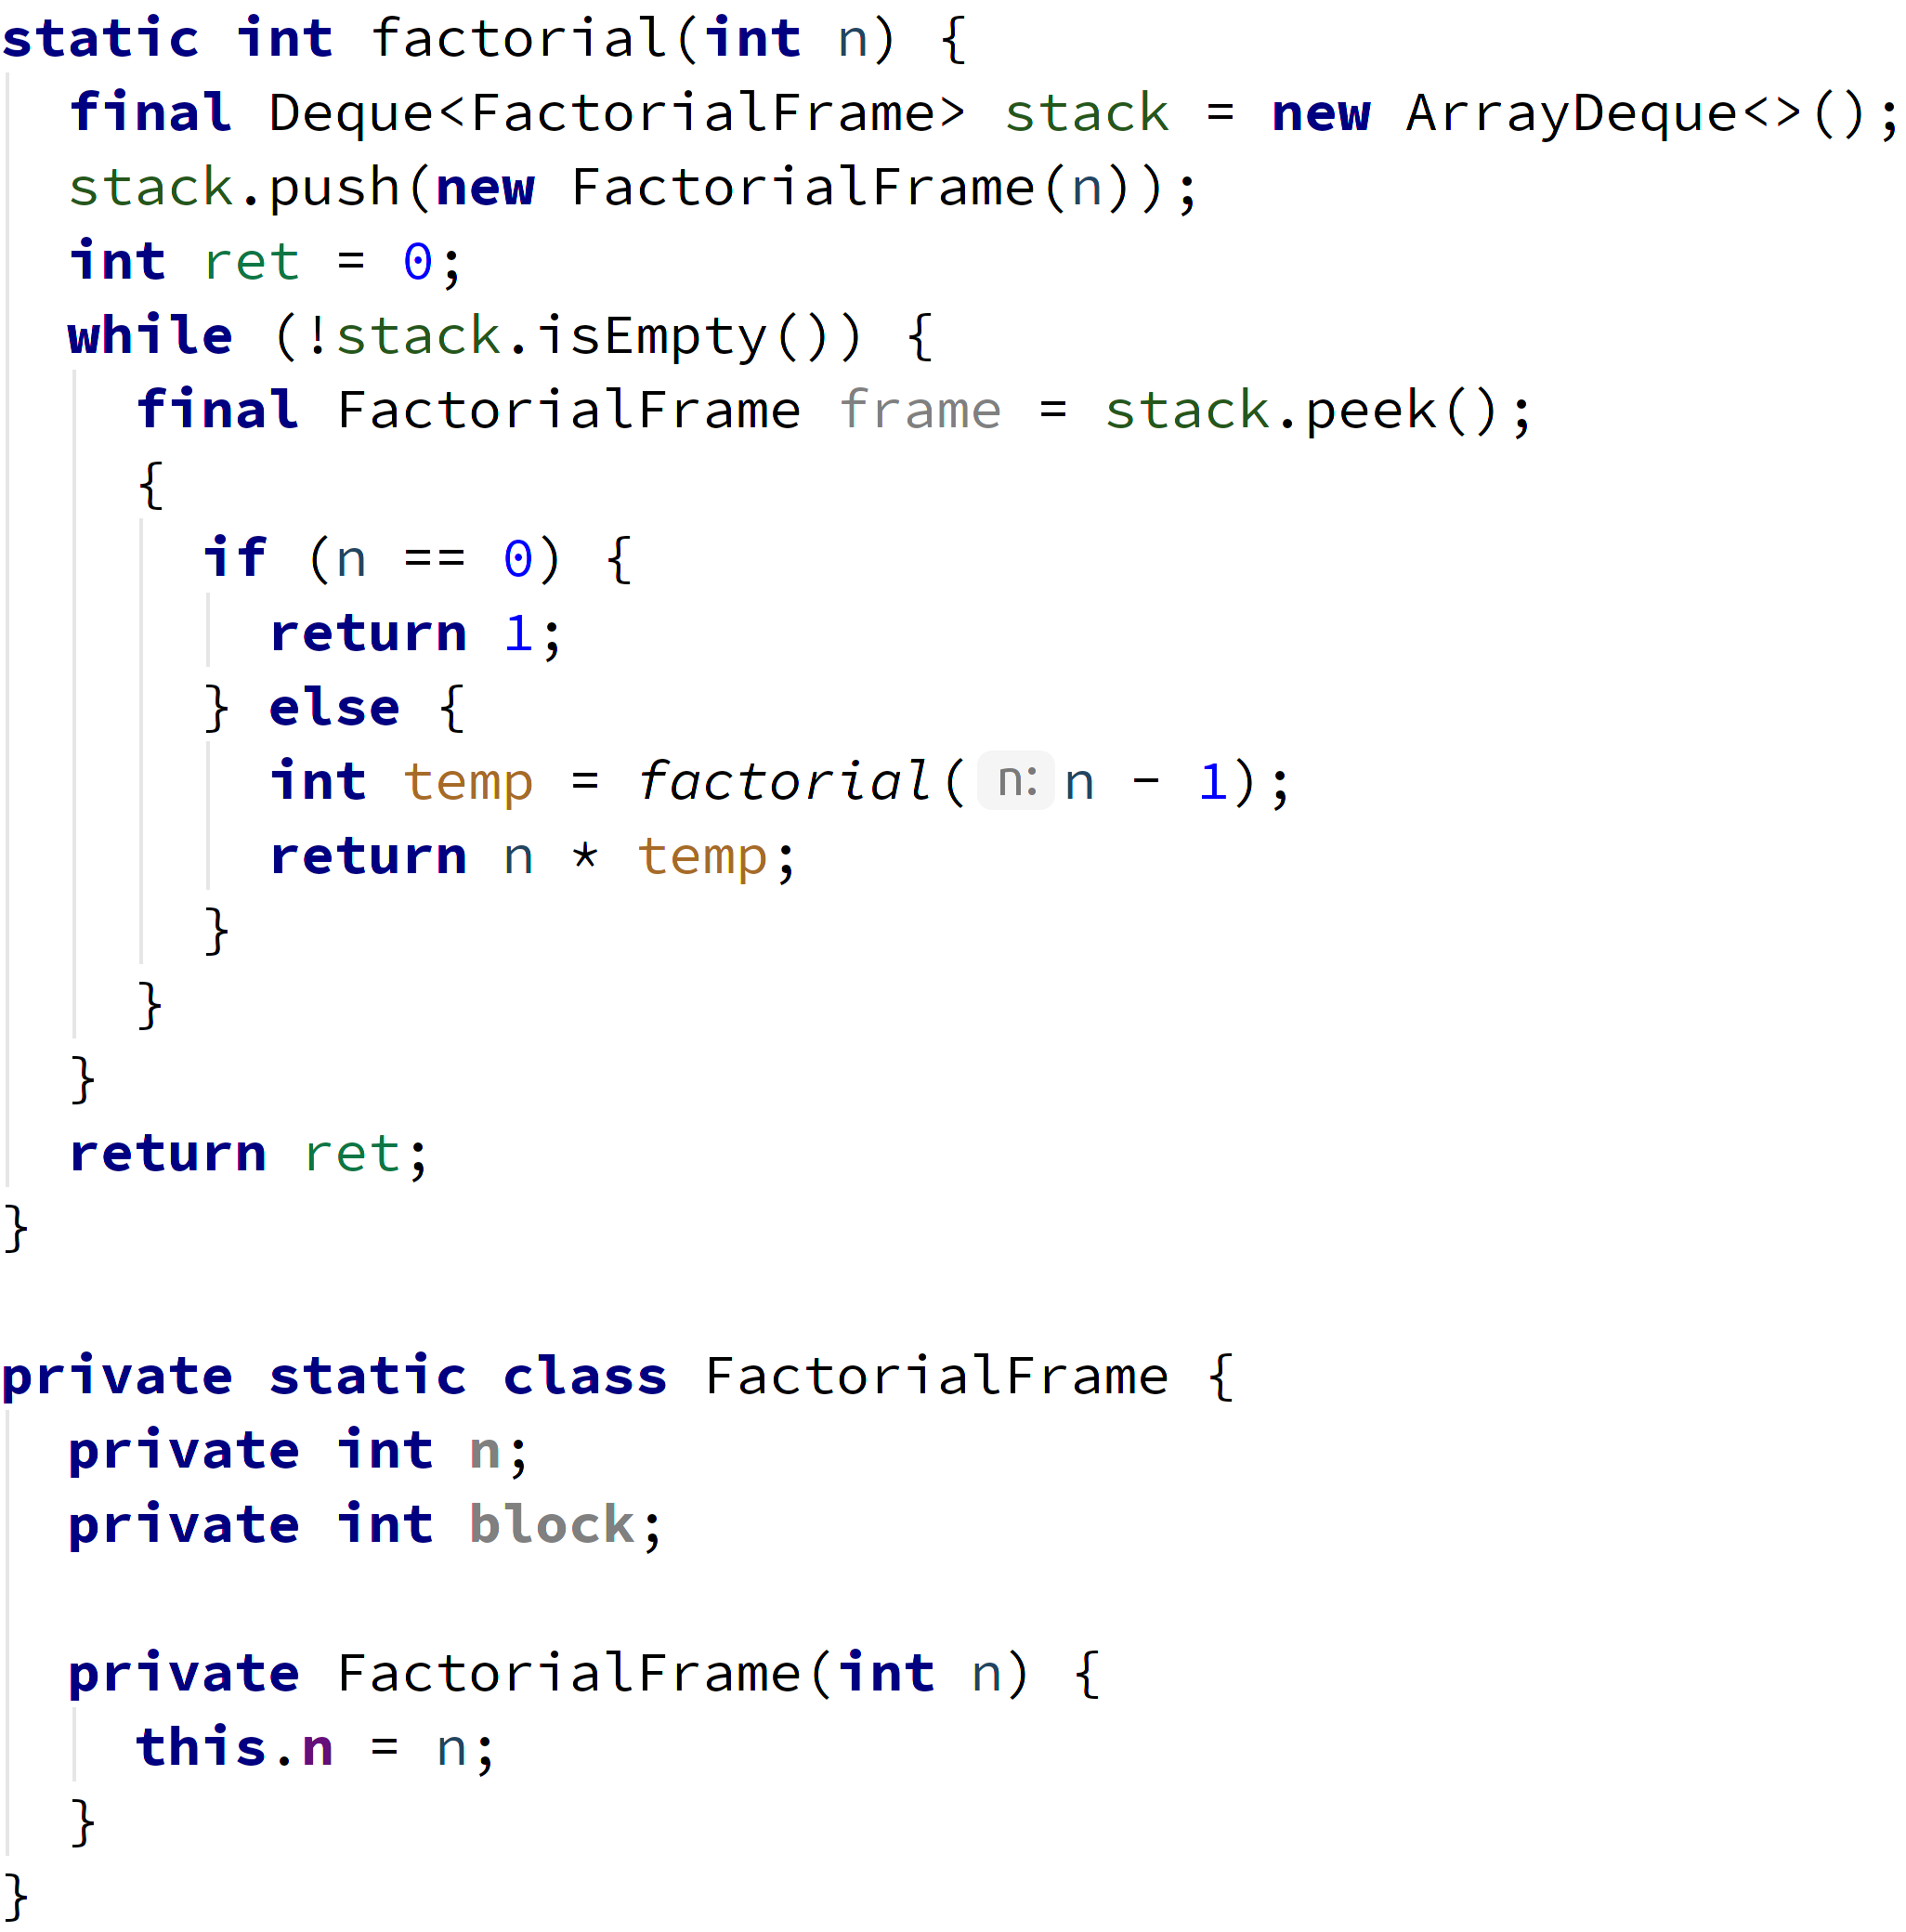
\includegraphics[height=2.456in]{../../../theses/diploma/src/img/incorporate-after-white-26.png}
%            \caption{După}
%        \end{subfigure}%
%        }\\
%        \caption{Includerea codului metodei în codul auxiliar}
%    \end{figure}
    \begin{itemize}
        \item Declararea unei stive explicite în program
        \item Adăugarea la stivă a unei înregistrări de activare ce reprezintă apelul metodei din exterior
        \item Declararea unei variabile \code{ret} ce reține valoarea întoarsă de apelul recursiv
        \item Includerea codului metodei într-o buclă \code{while} care ciclează până când se golește stiva
        \item Declararea în interiorul buclei \code{while} a unei variabile \code{frame}, inițializată la înregistrarea
        de activare din vârful stivei
        \item Adăugarea unei instructiuni \code{return ret;} care întoarce valoarea apelului exterior
    \end{itemize}
\end{frame}

\begin{frame}{Tratarea variabilelor locale}
% bullet: Inlocuire referintei la variabila
% bullet: Exemplu if factorial
% bullet: Inlocuirea declaratiilor variabilelor
% bullet: Exemplu: declaratie cu initializare
    \begin{itemize}
        \item Înlocuirea referințelor la variabile
        \item Înlocuirea declarațiilor de variabile locale
        \begin{figure}[htb]
            \begin{subfigure}[b]{.48\textwidth}
                \centering
                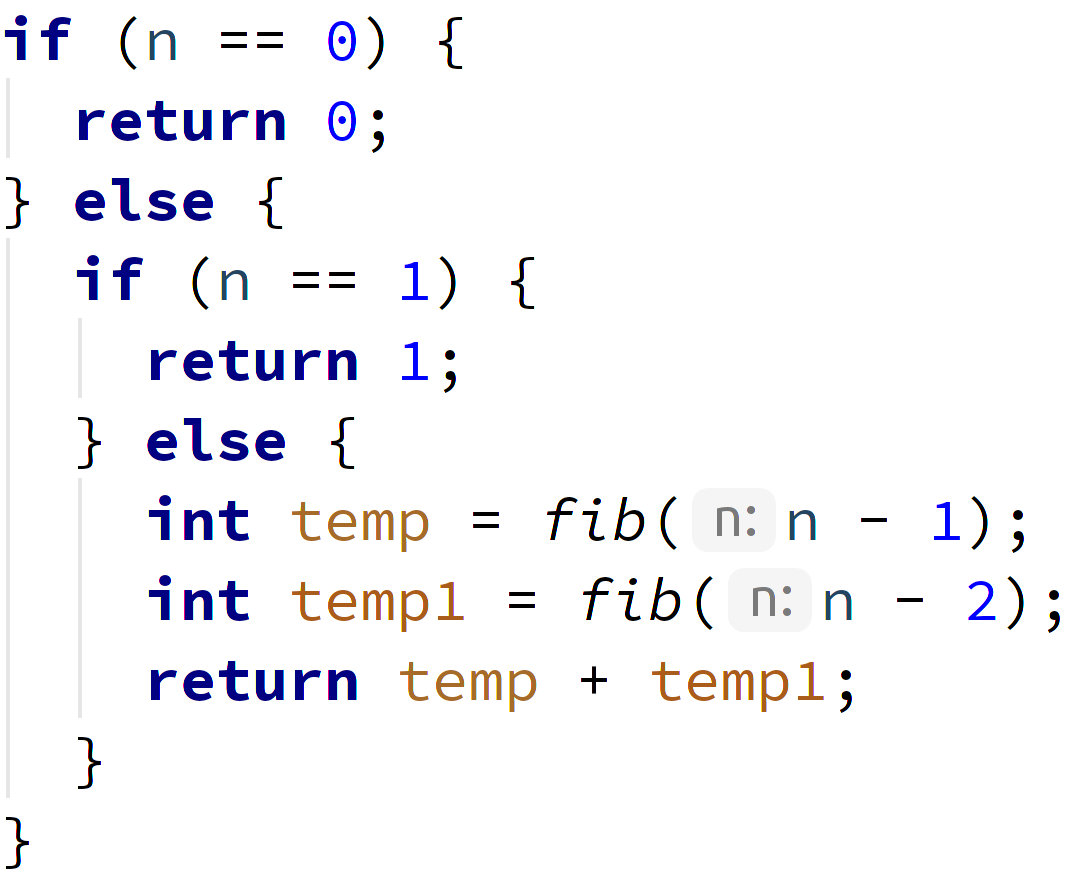
\includegraphics[height=1.65in]{img/ref-var-before.png}
                \caption{Înainte}
            \end{subfigure}
            \begin{subfigure}[b]{.48\textwidth}
                \centering
                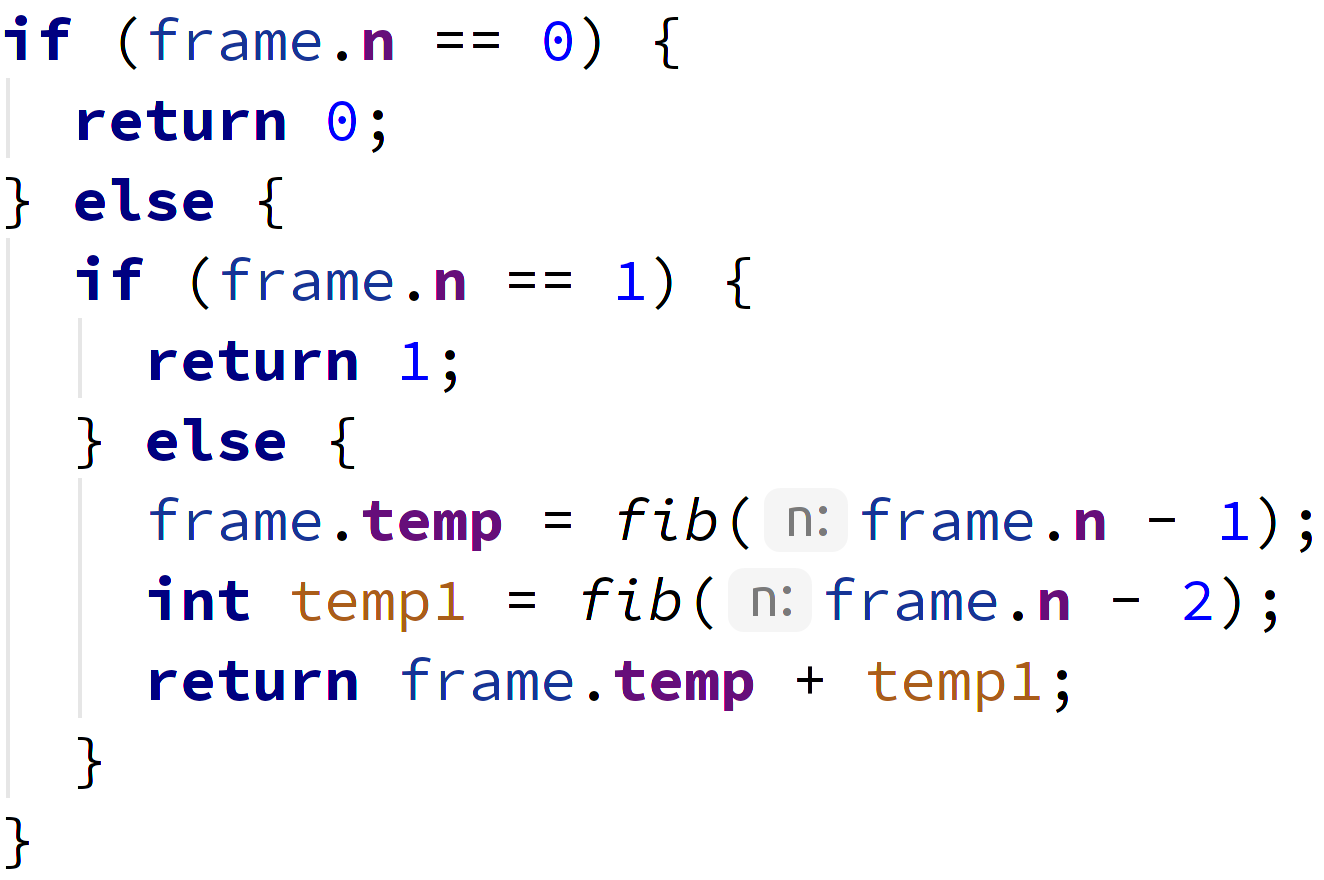
\includegraphics[height=1.65in]{img/ref-var-after.png}
                \caption{După}
            \end{subfigure}
        \end{figure}
    \end{itemize}
\end{frame}

%\begin{frame}{Înlocuirea declarațiilor având inițializare cu accese la câmpul din cadrul de stivă}
%    \begin{figure}[htb]
%        \makebox[\linewidth][c]{%
%        \begin{subfigure}[b]{.5\textwidth}
%            \centering
%            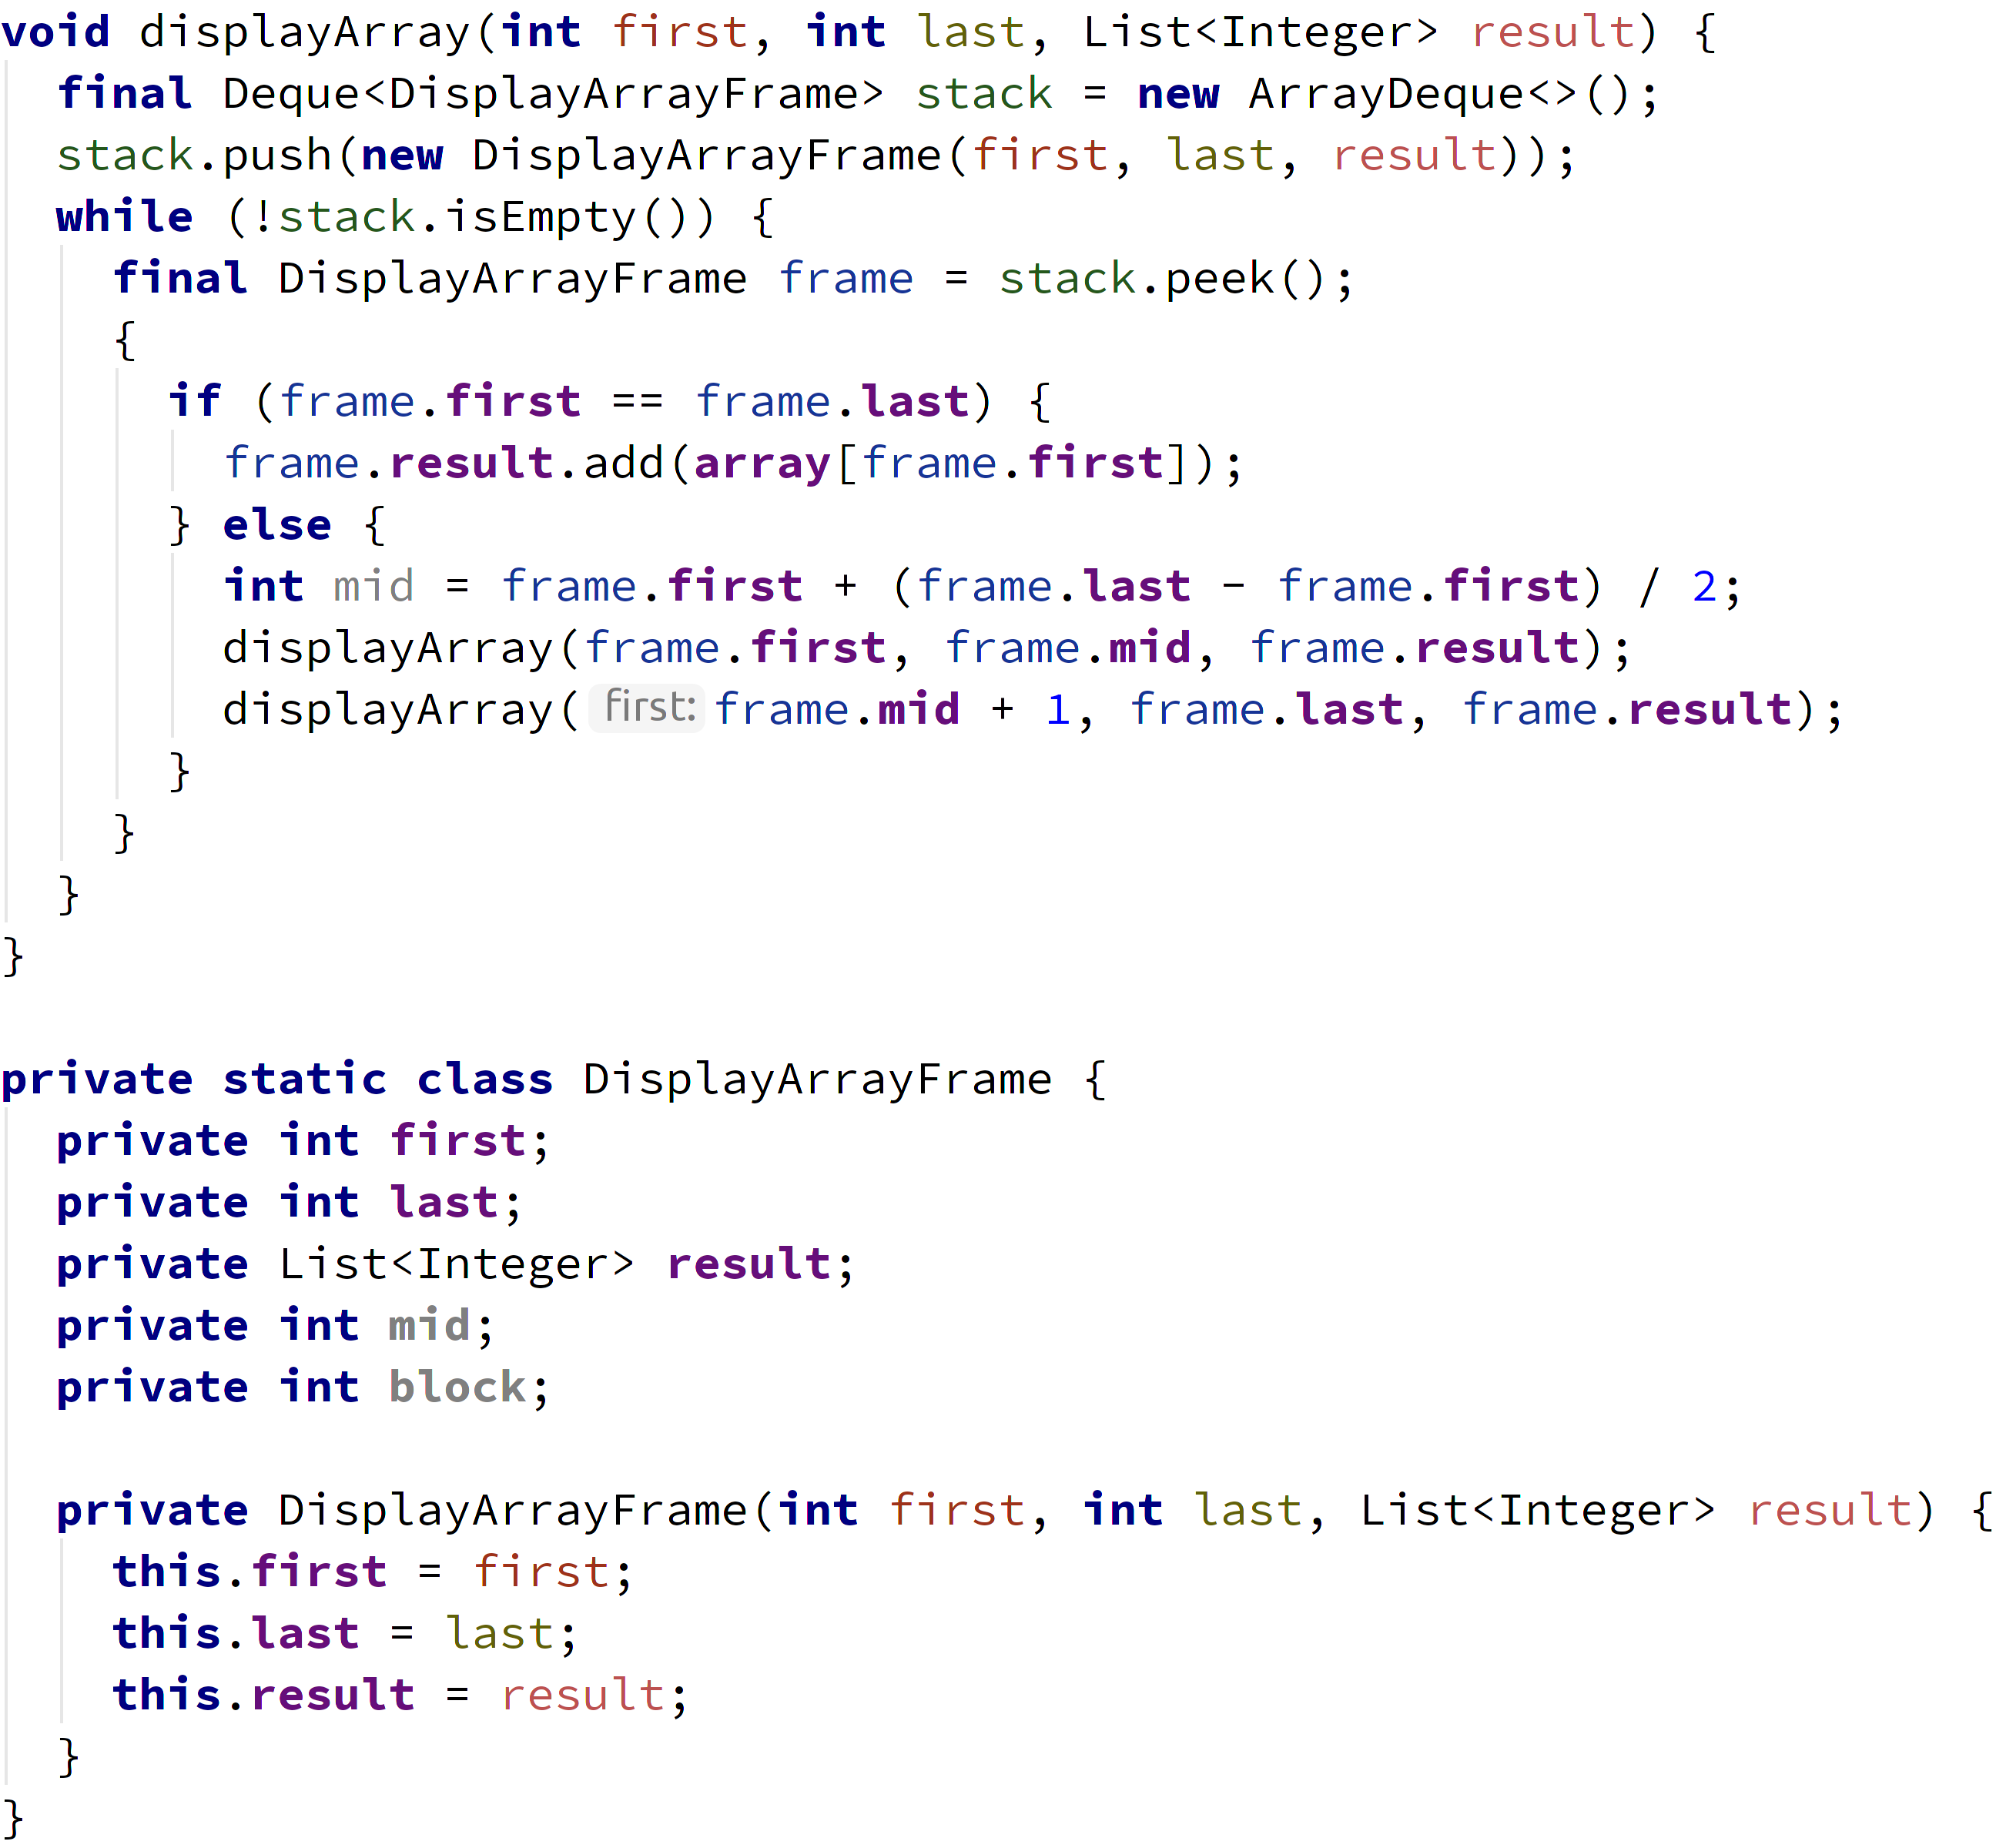
\includegraphics[width=2.1in]{../../../theses/diploma/src/img/replace-declaration-before-white-30.png}
%            \caption{Înainte}
%        \end{subfigure}%
%        \begin{subfigure}[b]{.5\textwidth}
%            \centering
%            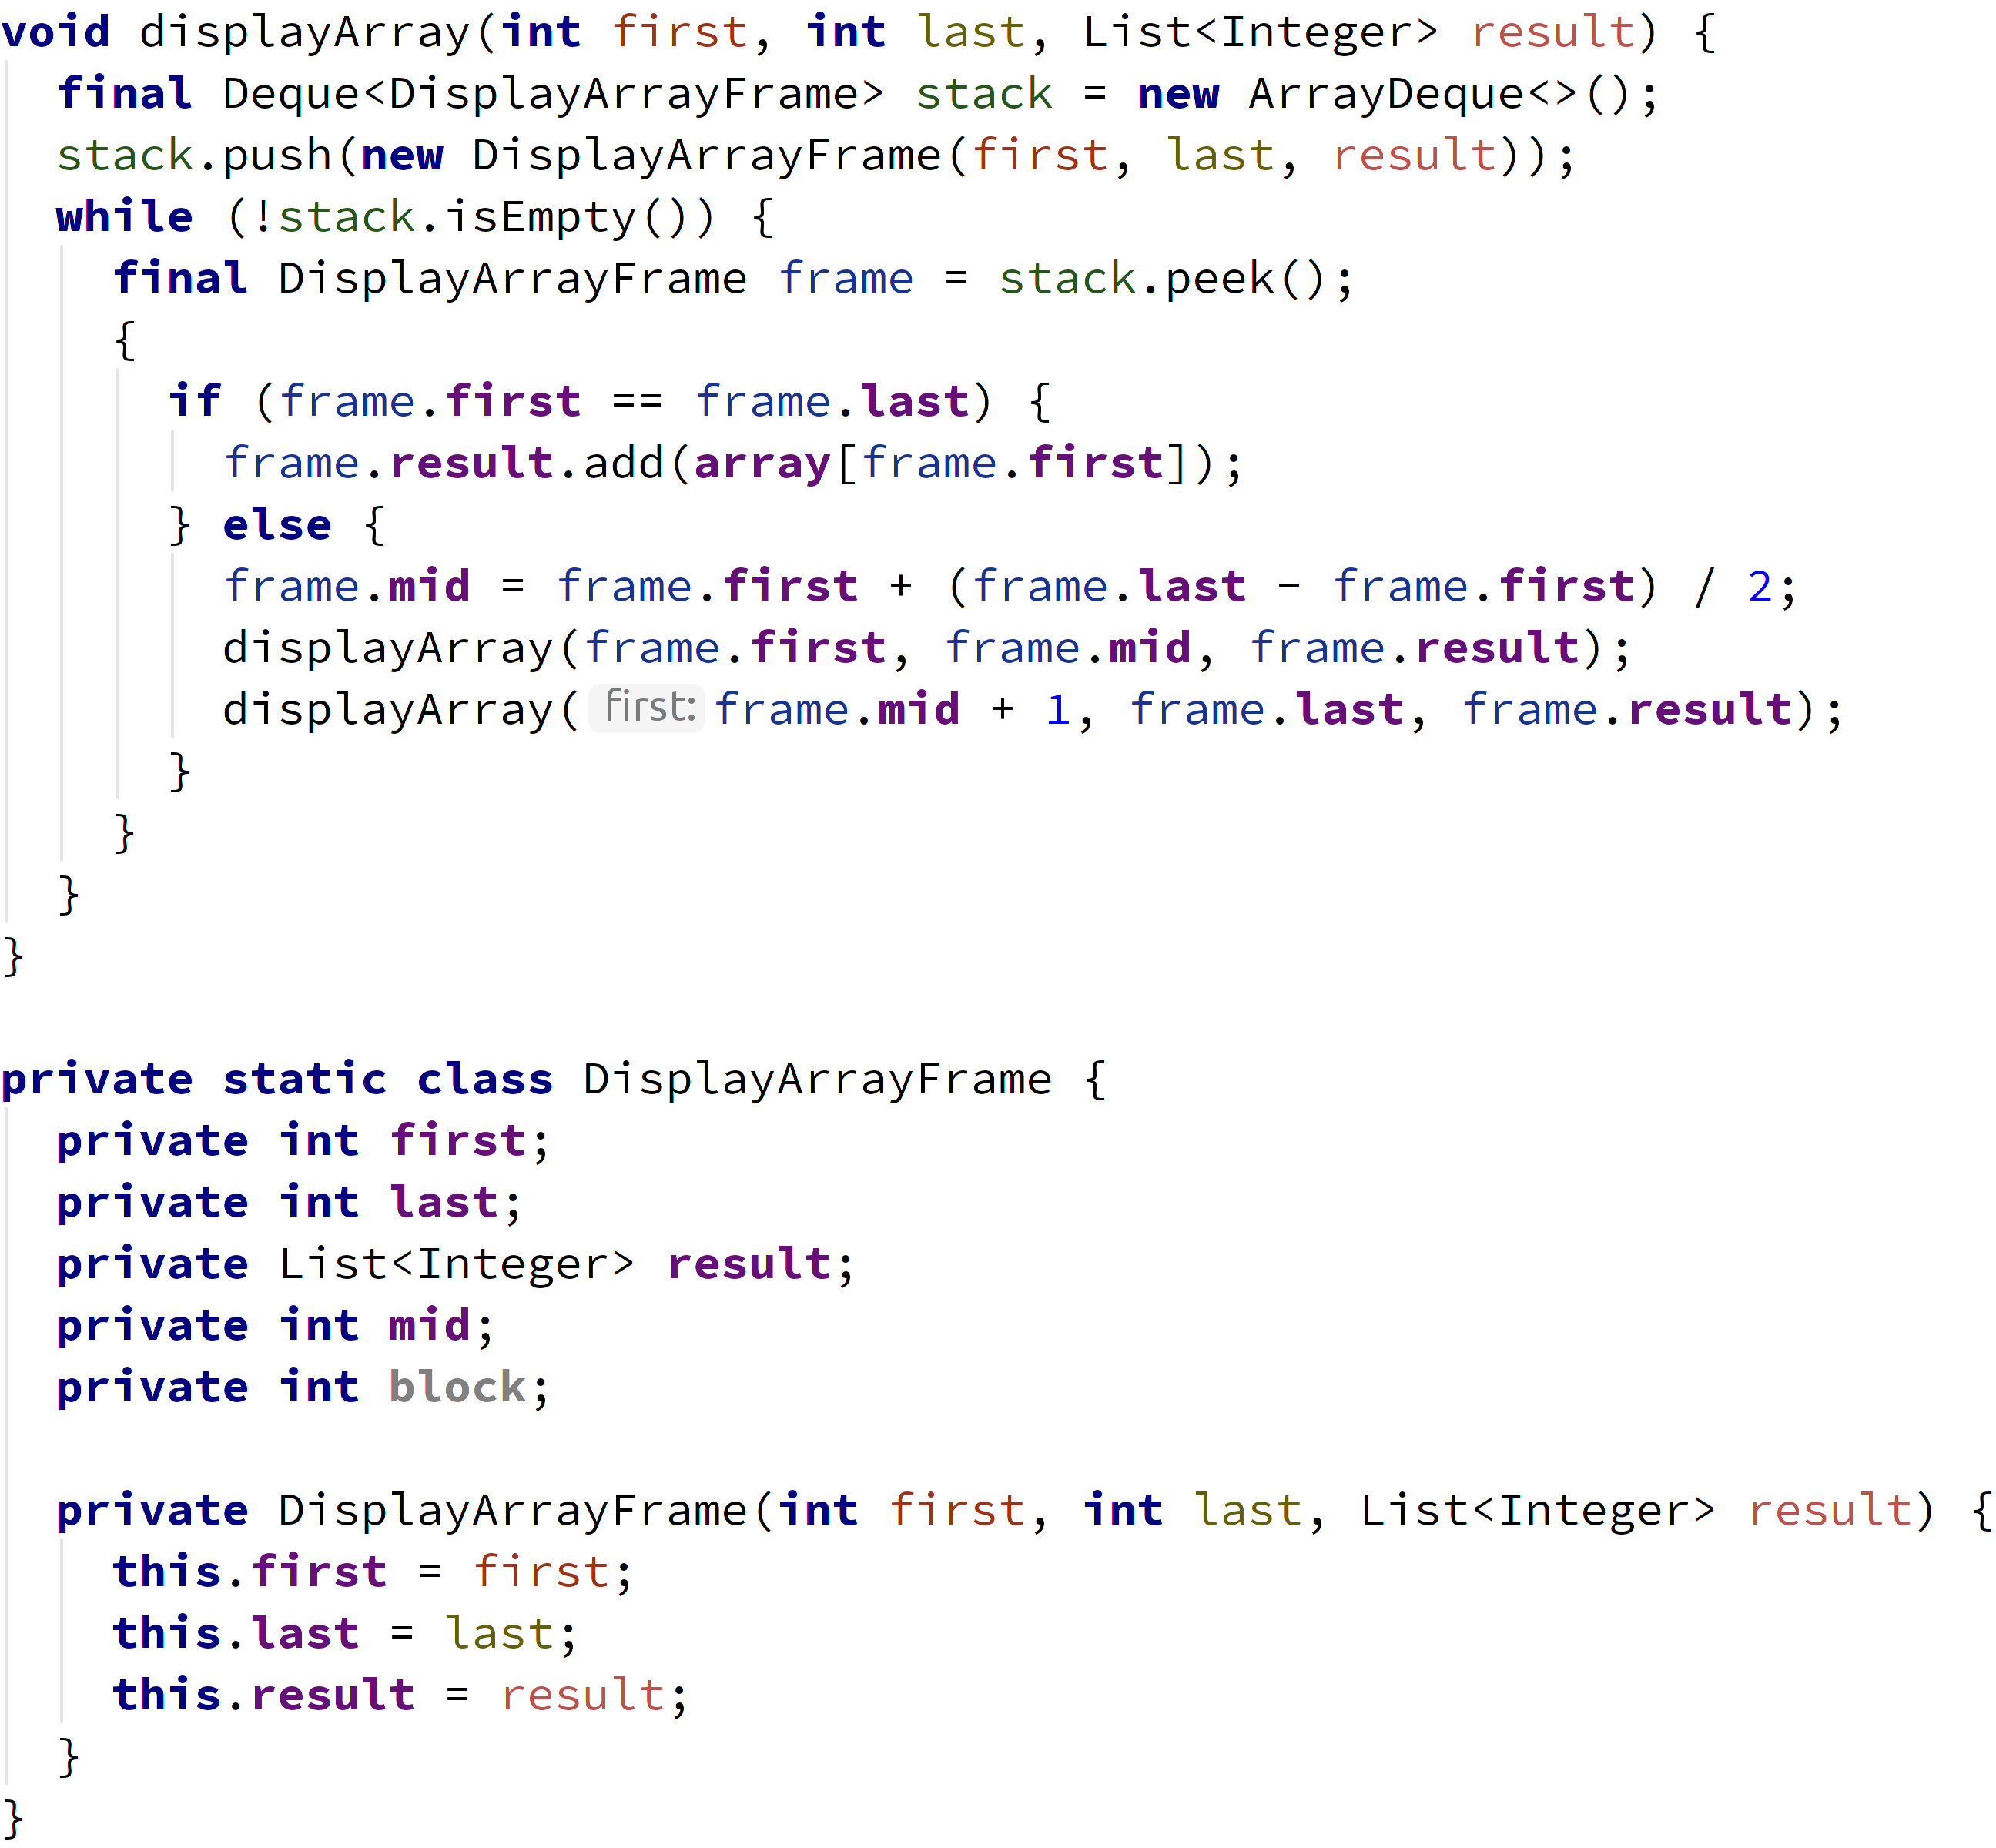
\includegraphics[width=2.1in]{../../../theses/diploma/src/img/replace-declaration-after-white-30.png}
%            \caption{După}
%        \end{subfigure}%
%        }\\
%    \end{figure}
%\end{frame}

\begin{frame}{Generarea grafului fluxului de control (Instrucțiunea \code{if})}
    \begin{figure}[htb]
        \centering
        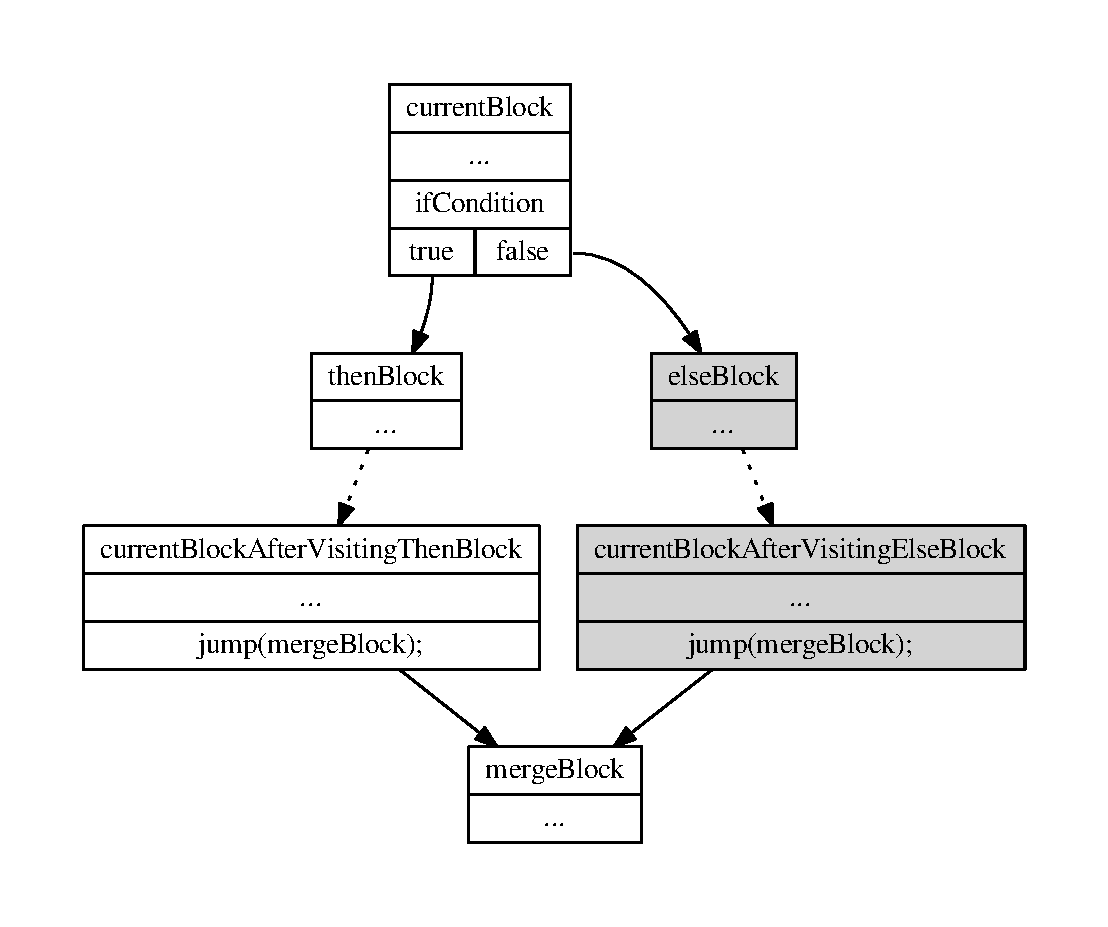
\includegraphics[width=.7\textwidth]{../../../theses/diploma/src/graph/if.pdf}
    \end{figure}
\end{frame}

\begin{frame}{Generarea grafului fluxului de control (Instrucțiuni de ciclare)}
    \begin{figure}[htb]
        \begin{subfigure}[b]{0.32\textwidth}
            \centering
            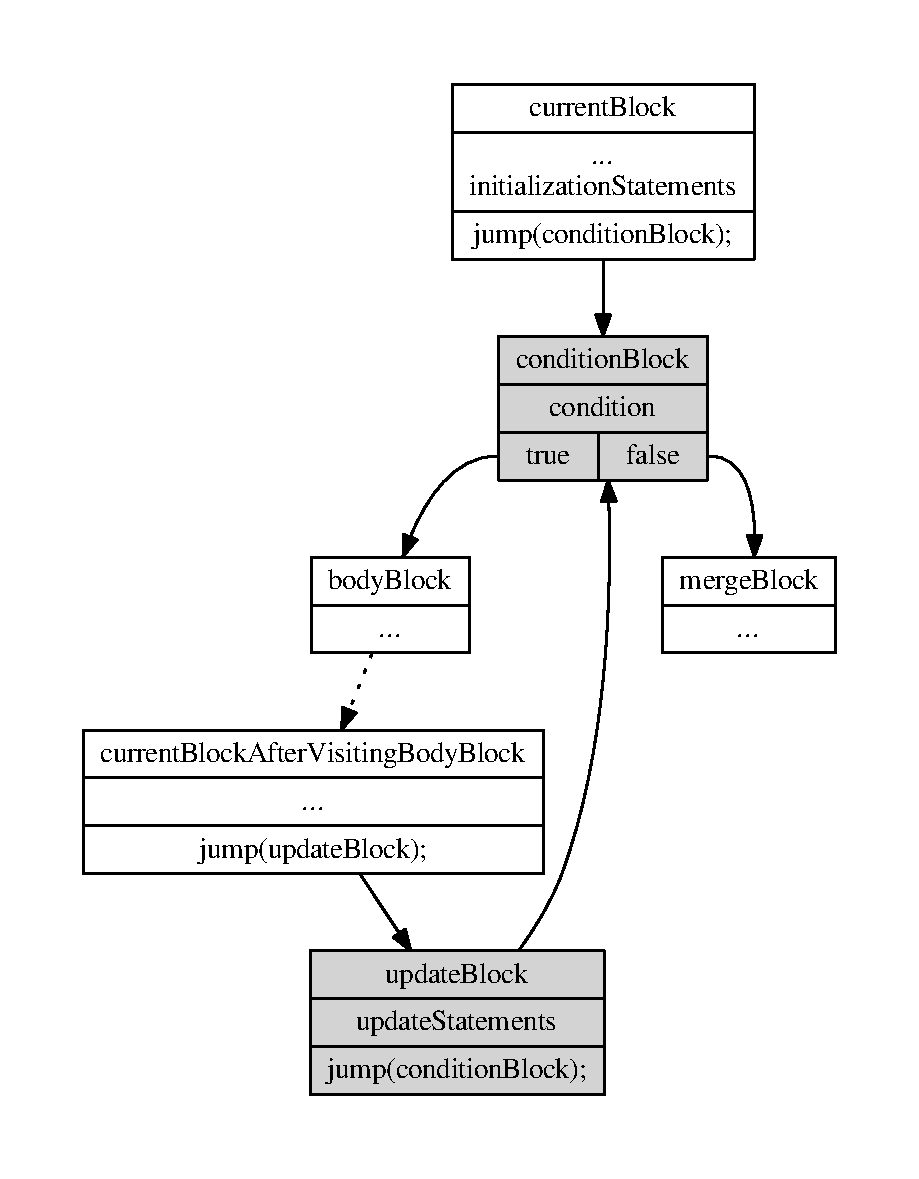
\includegraphics[width=\textwidth]{../../../theses/diploma/src/graph/for.pdf}
            \caption{\code{for}}
        \end{subfigure}
        \hfill
        \begin{subfigure}[b]{0.32\textwidth}
            \centering
            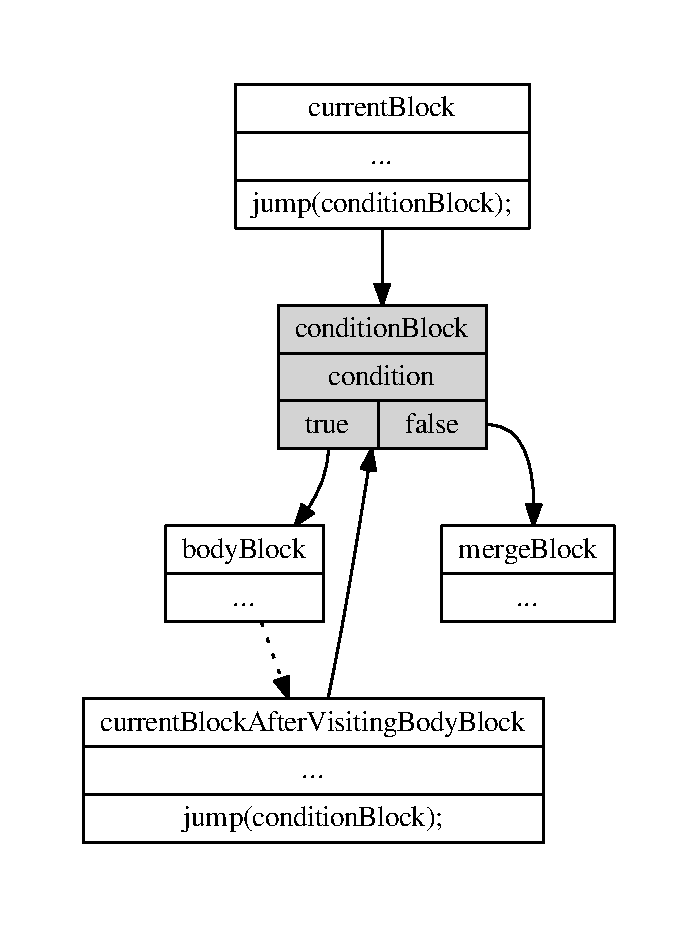
\includegraphics[width=\textwidth]{../../../theses/diploma/src/graph/while.pdf}
            \caption{\code{while}}
        \end{subfigure}
        \hfill
        \begin{subfigure}[b]{0.32\textwidth}
            \centering
            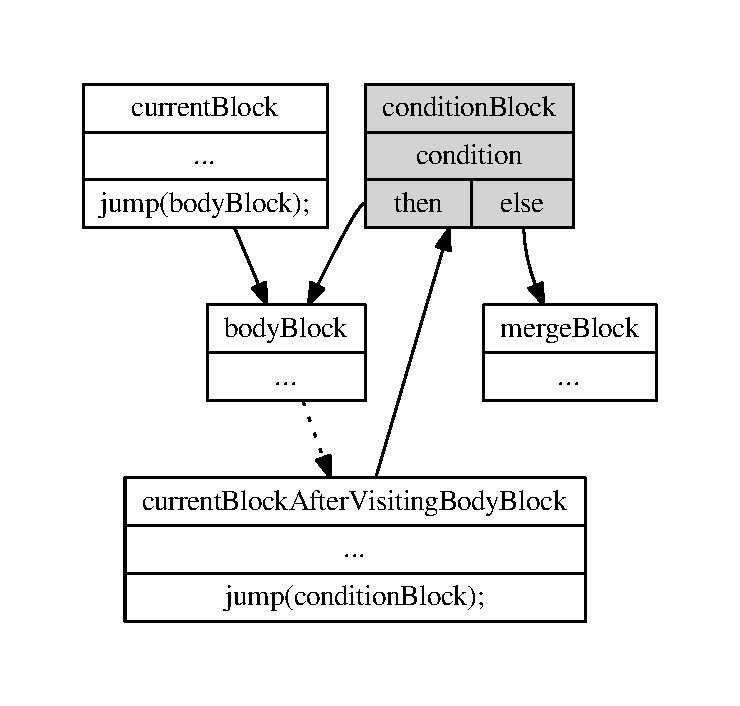
\includegraphics[width=\textwidth]{../../../theses/diploma/src/graph/do-while.pdf}
            \caption{\code{do-while}}
        \end{subfigure}
    \end{figure}
\end{frame}

\begin{frame}{Generarea grafului fluxului de control (Apelul recursiv)}
    Tratarea apelului recursiv presupune:
    \begin{itemize}
        \item Înlocuirea sa cu adăugarea unei noi înregistrări de activare în vârful stivei, inițializată cu
        expresiile folosite ca parametri actuali ai apelului
        \item Crearea unui nou bloc de bază în graful fluxului de control
        \item Adăugarea unui salt necondiționat din blocul curent la noul bloc creat
        \item Setarea blocului curent la blocul nou creat
    \end{itemize}
\end{frame}

\begin{frame}{Generarea grafului fluxului de control (Exemplu)}
    \begin{figure}[htb]
        \begin{subfigure}{.42\textwidth}
            \centering
            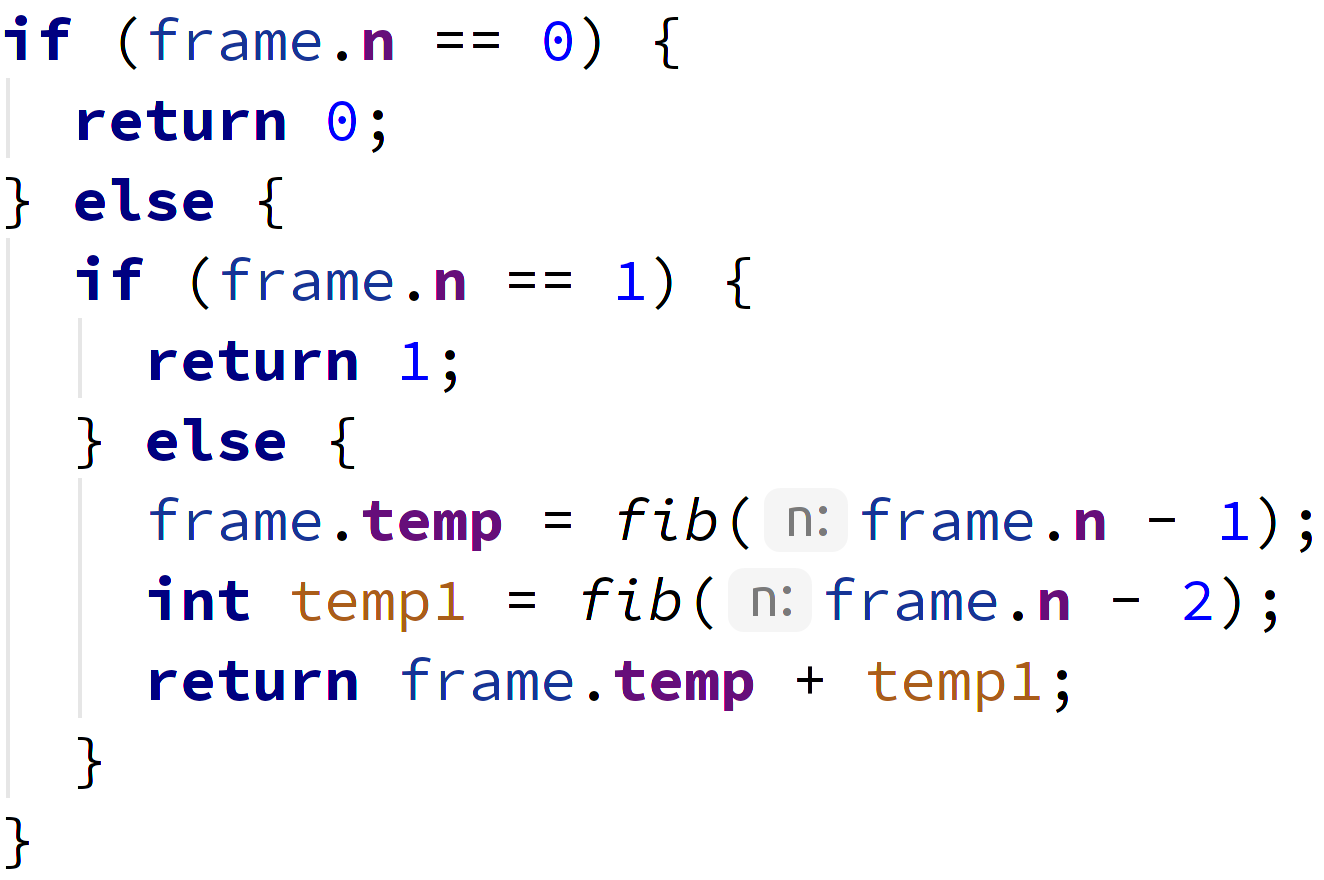
\includegraphics[width=\textwidth]{img/ref-var-after.png}
        \end{subfigure}
        \hfill
        \begin{subfigure}{.42\textwidth}
            \centering
            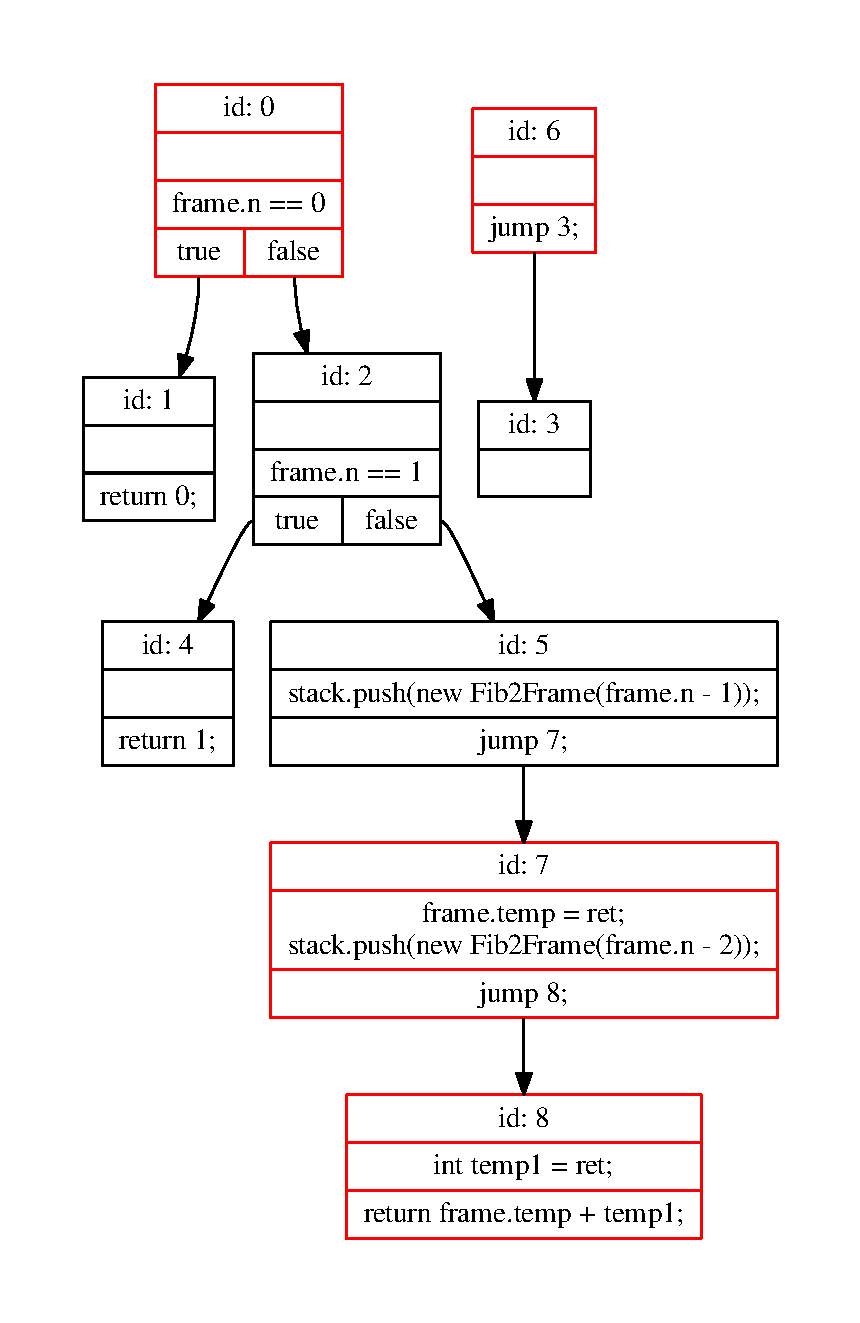
\includegraphics[width=\textwidth]{../../../theses/diploma/src/graph/cfg.pdf}
        \end{subfigure}
    \end{figure}
\end{frame}

\begin{frame}{Eliminarea blocurilor triviale (înainte)}
% eventual un exemplu scris de mine, care e mai simplu
    \begin{figure}[htb]
        \centering
        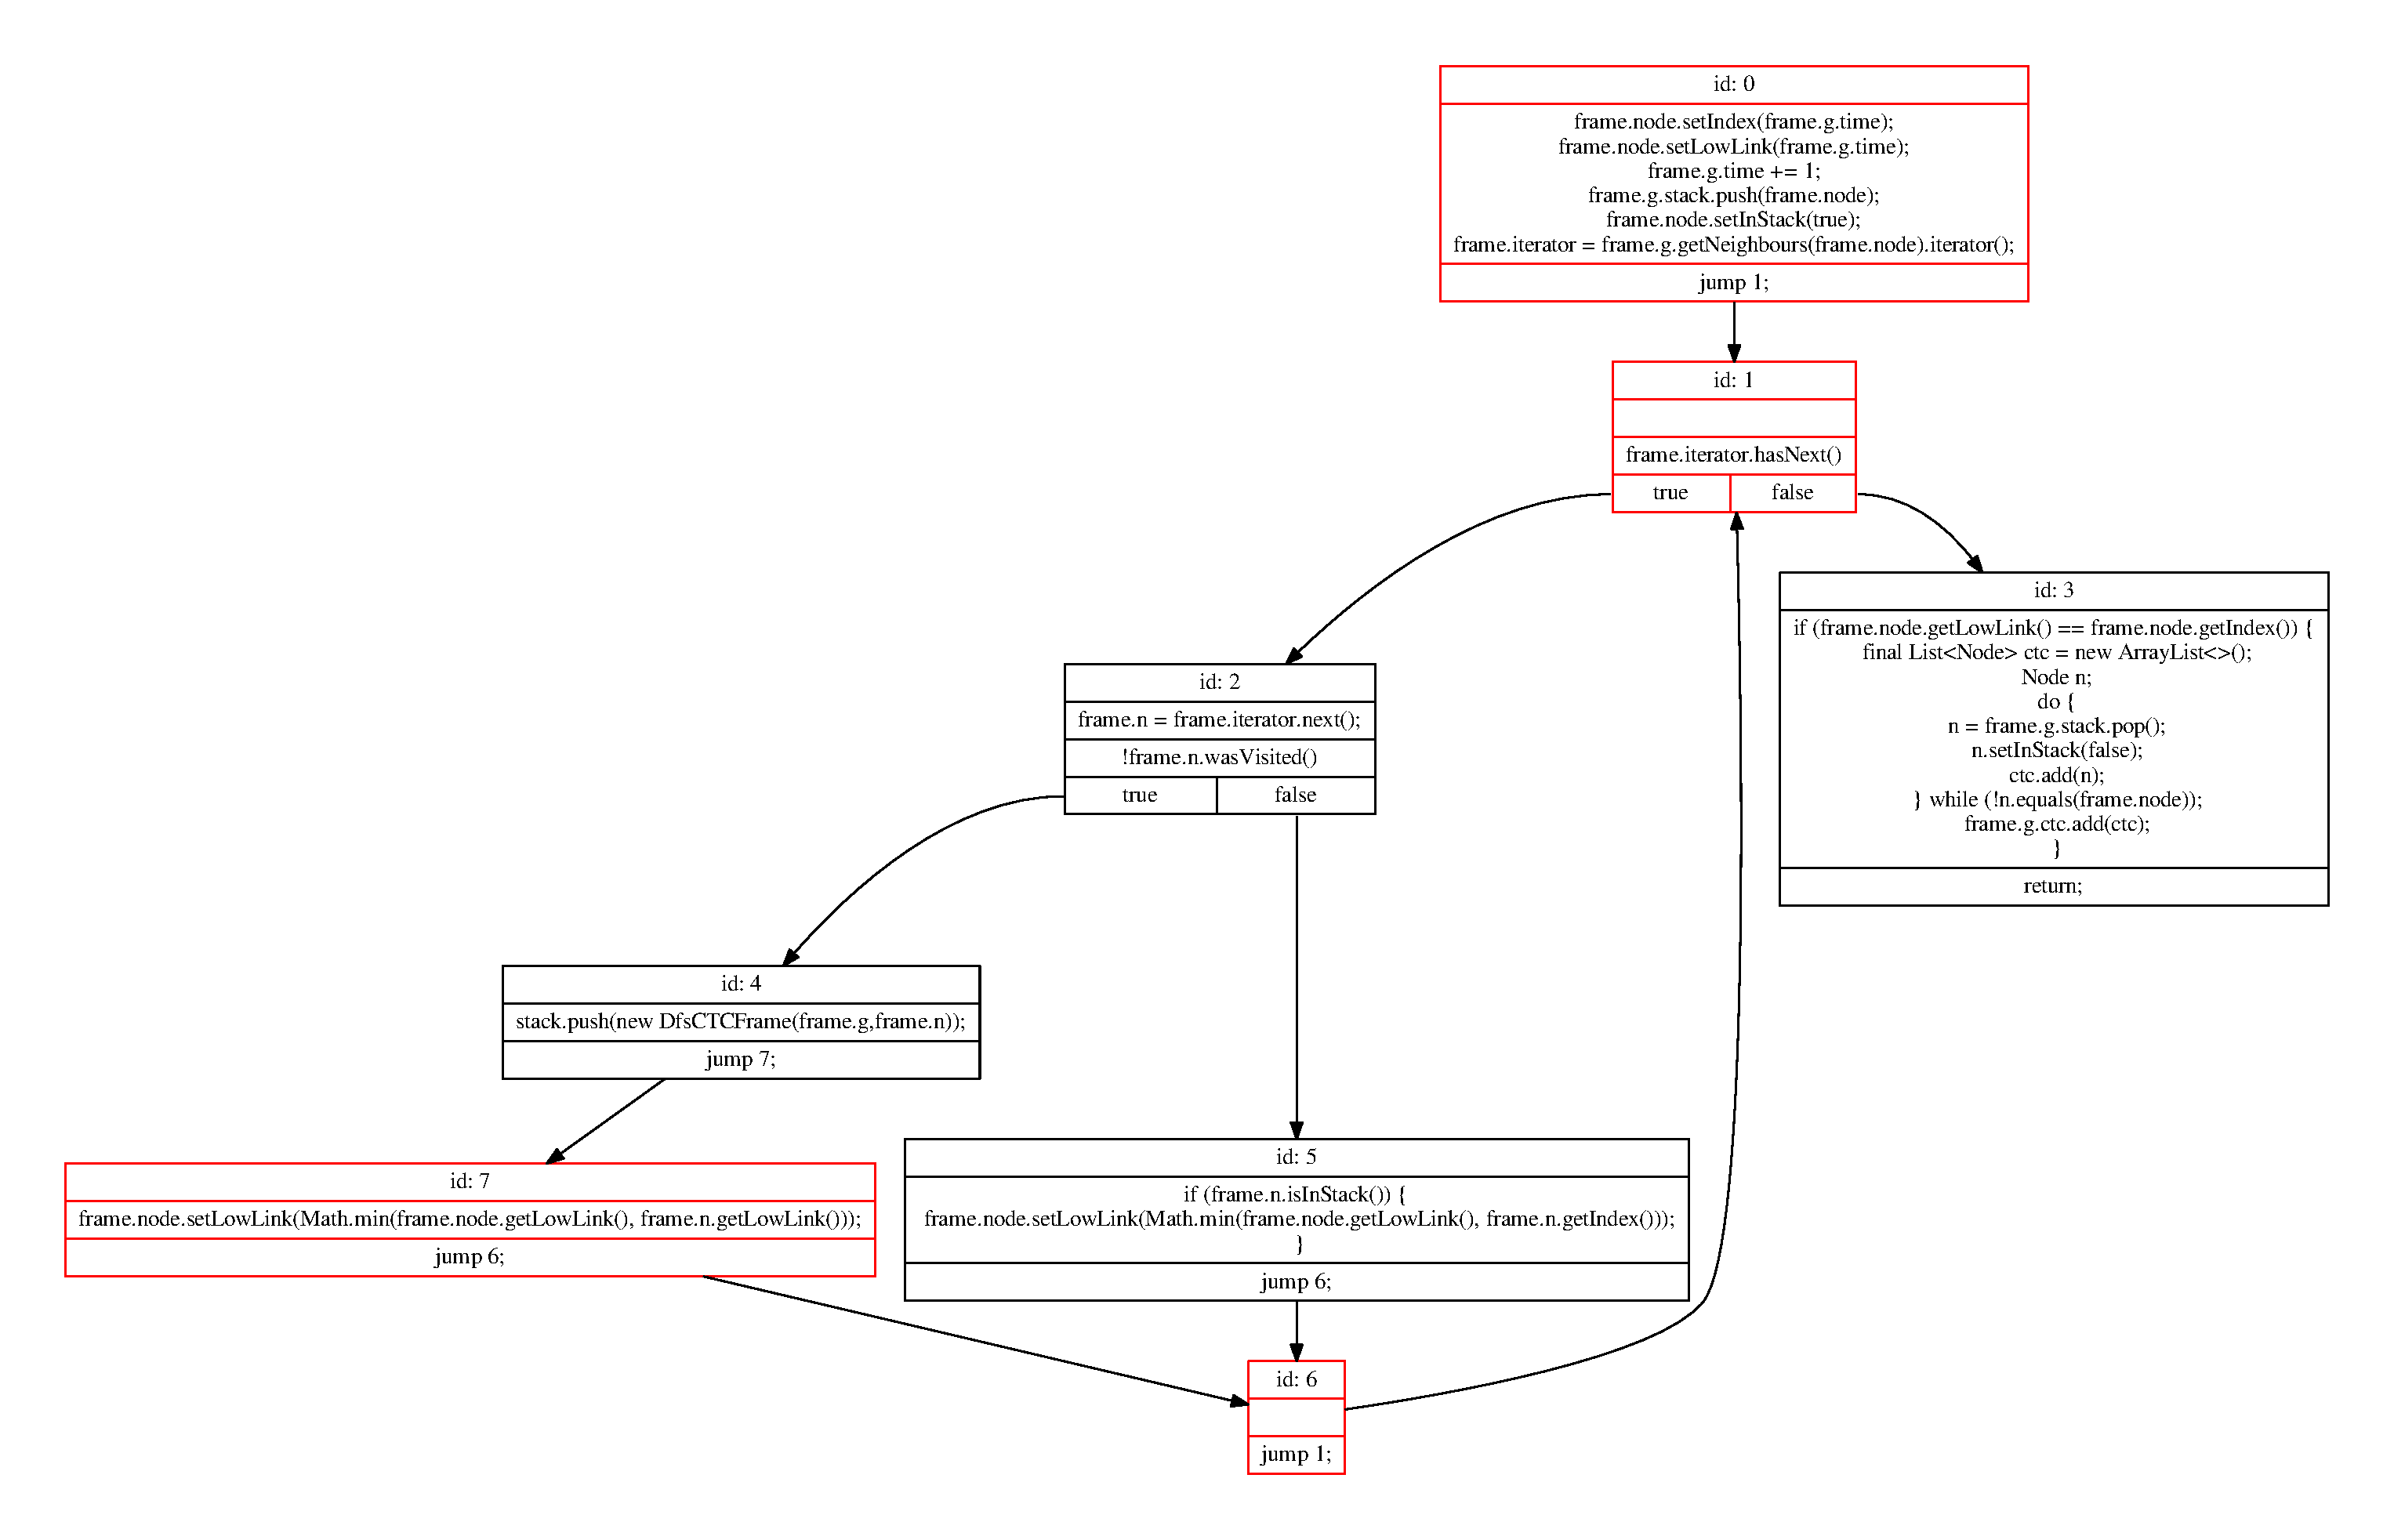
\includegraphics[width=\linewidth]{../../../theses/diploma/src/graph/trivial-before.pdf}
    \end{figure}
    \begin{figure}[htb]
        \centering
        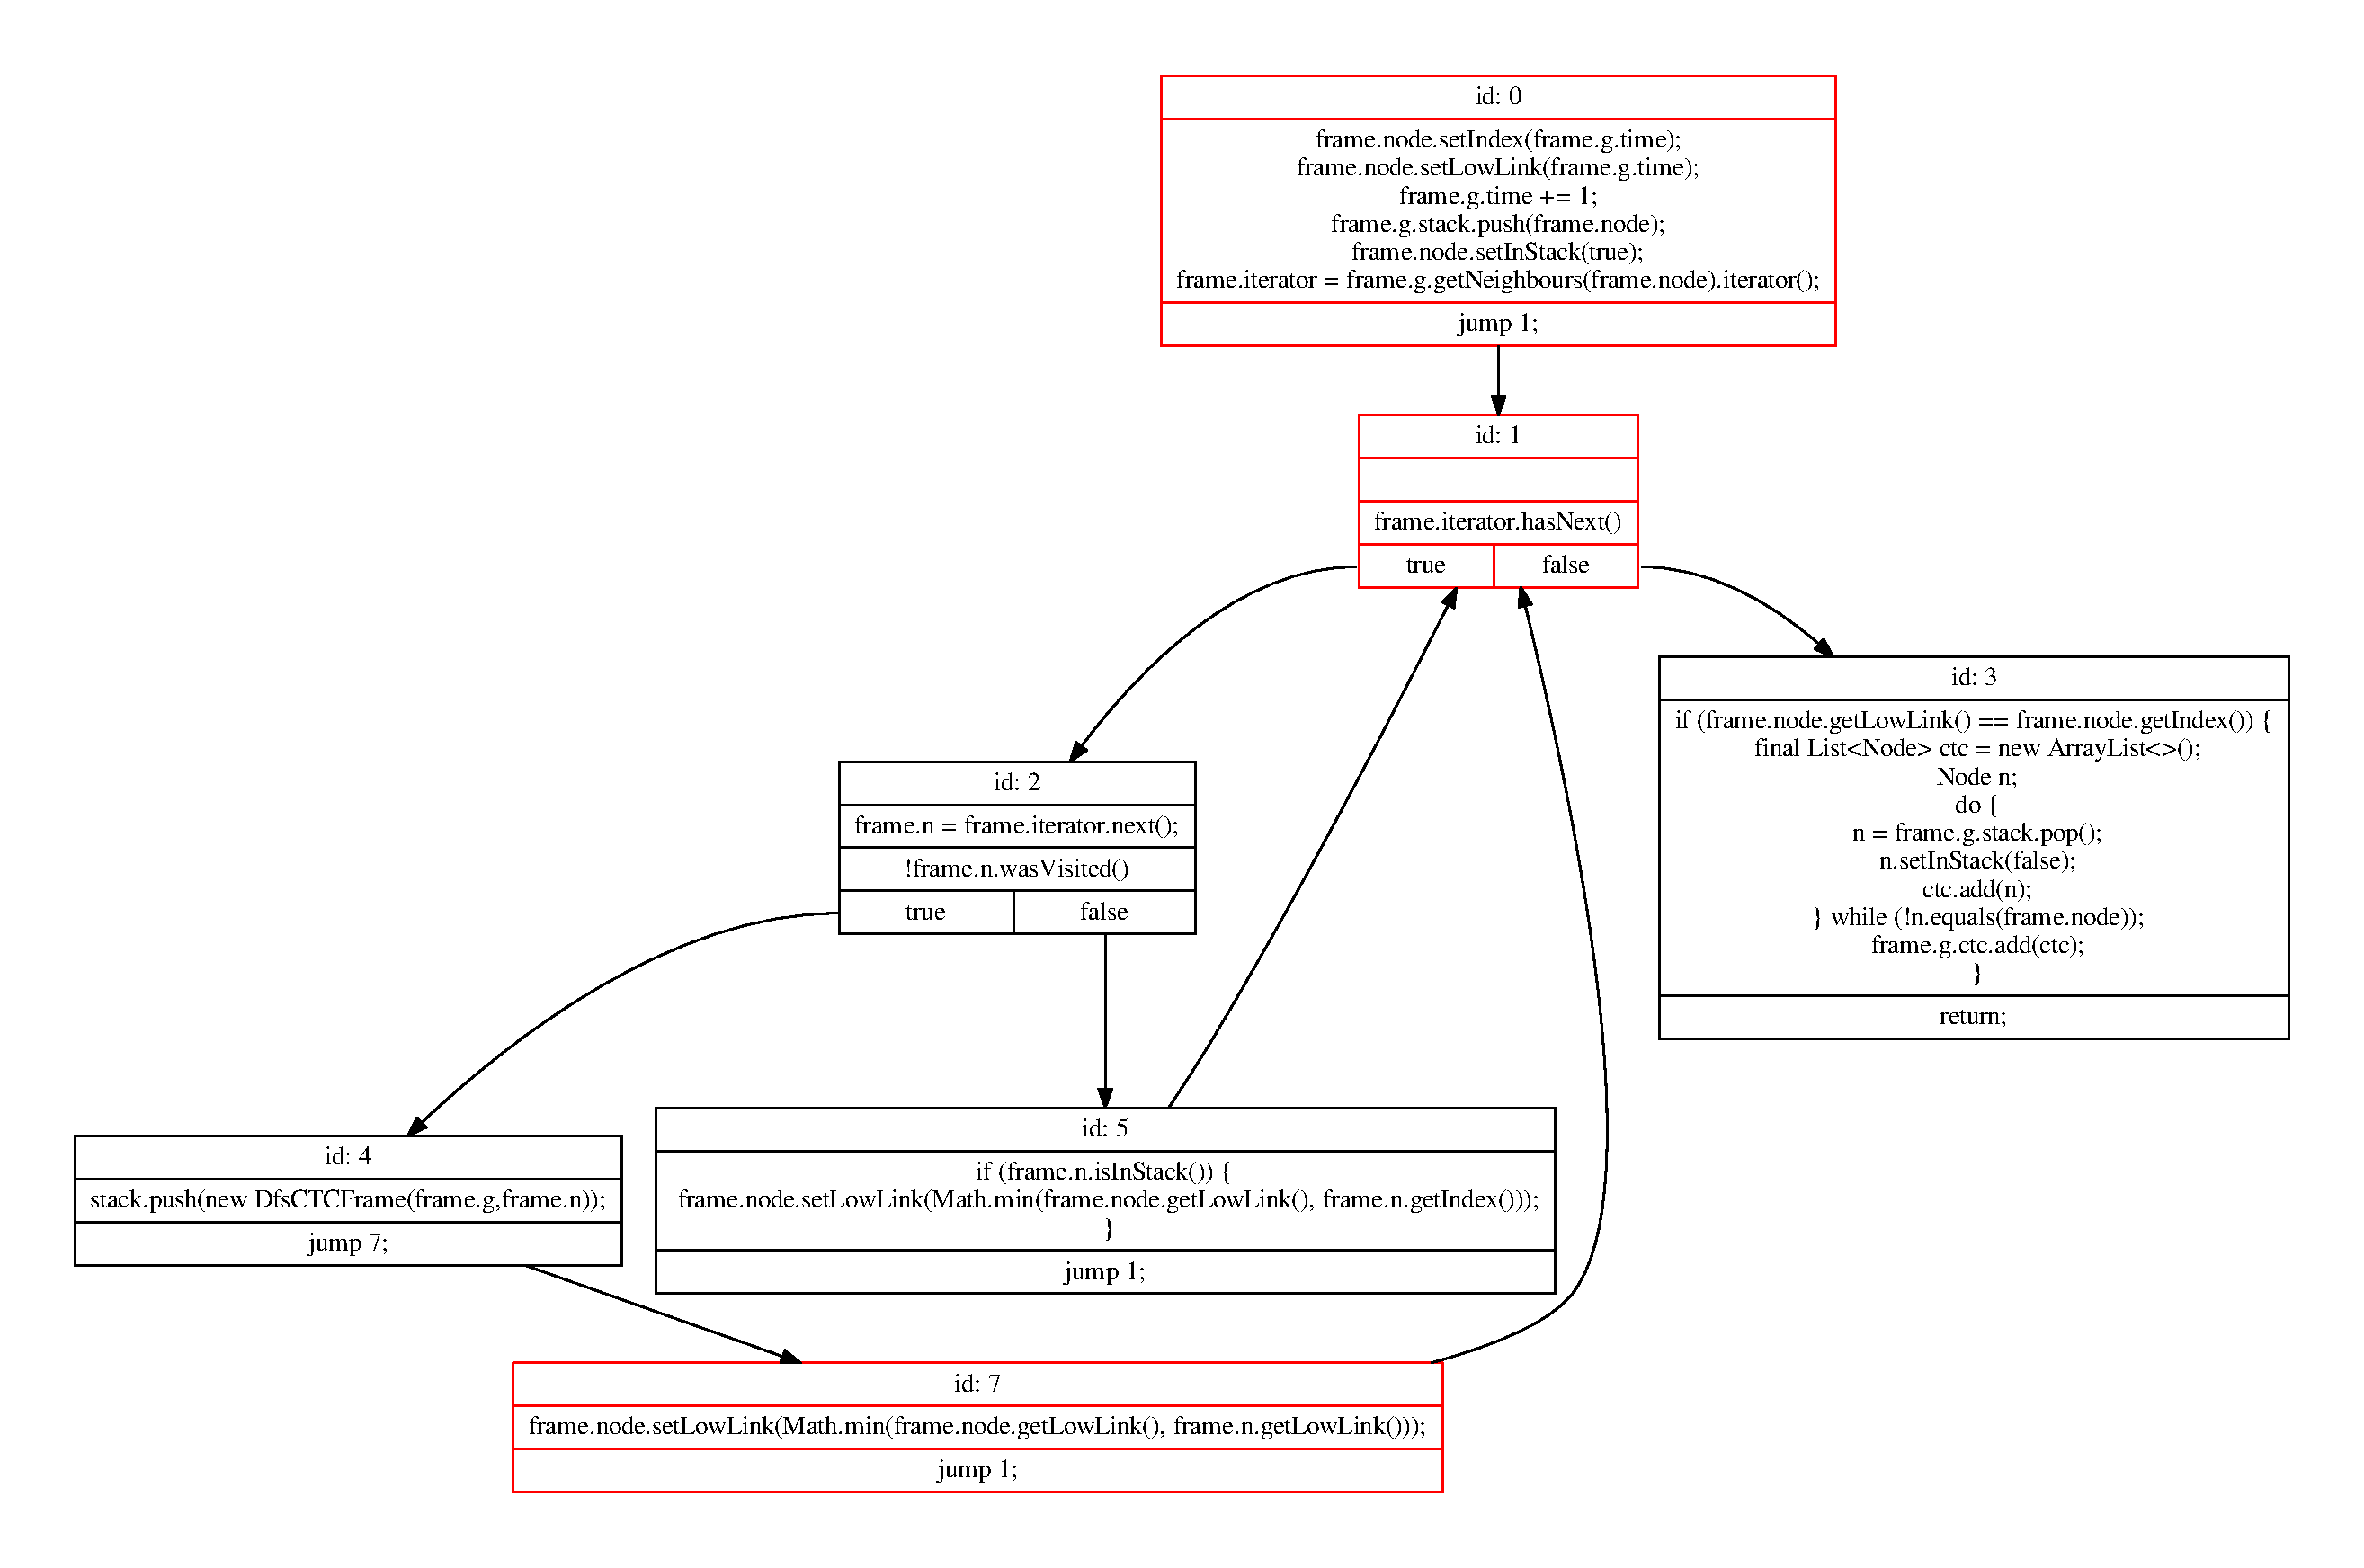
\includegraphics[width=\linewidth]{../../../theses/diploma/src/graph/trivial-after.pdf}
        \caption{After}
    \end{figure}
\end{frame}

\begin{frame}{Eliminarea blocurilor triviale (după)}
    \begin{figure}[htb]
        \centering
        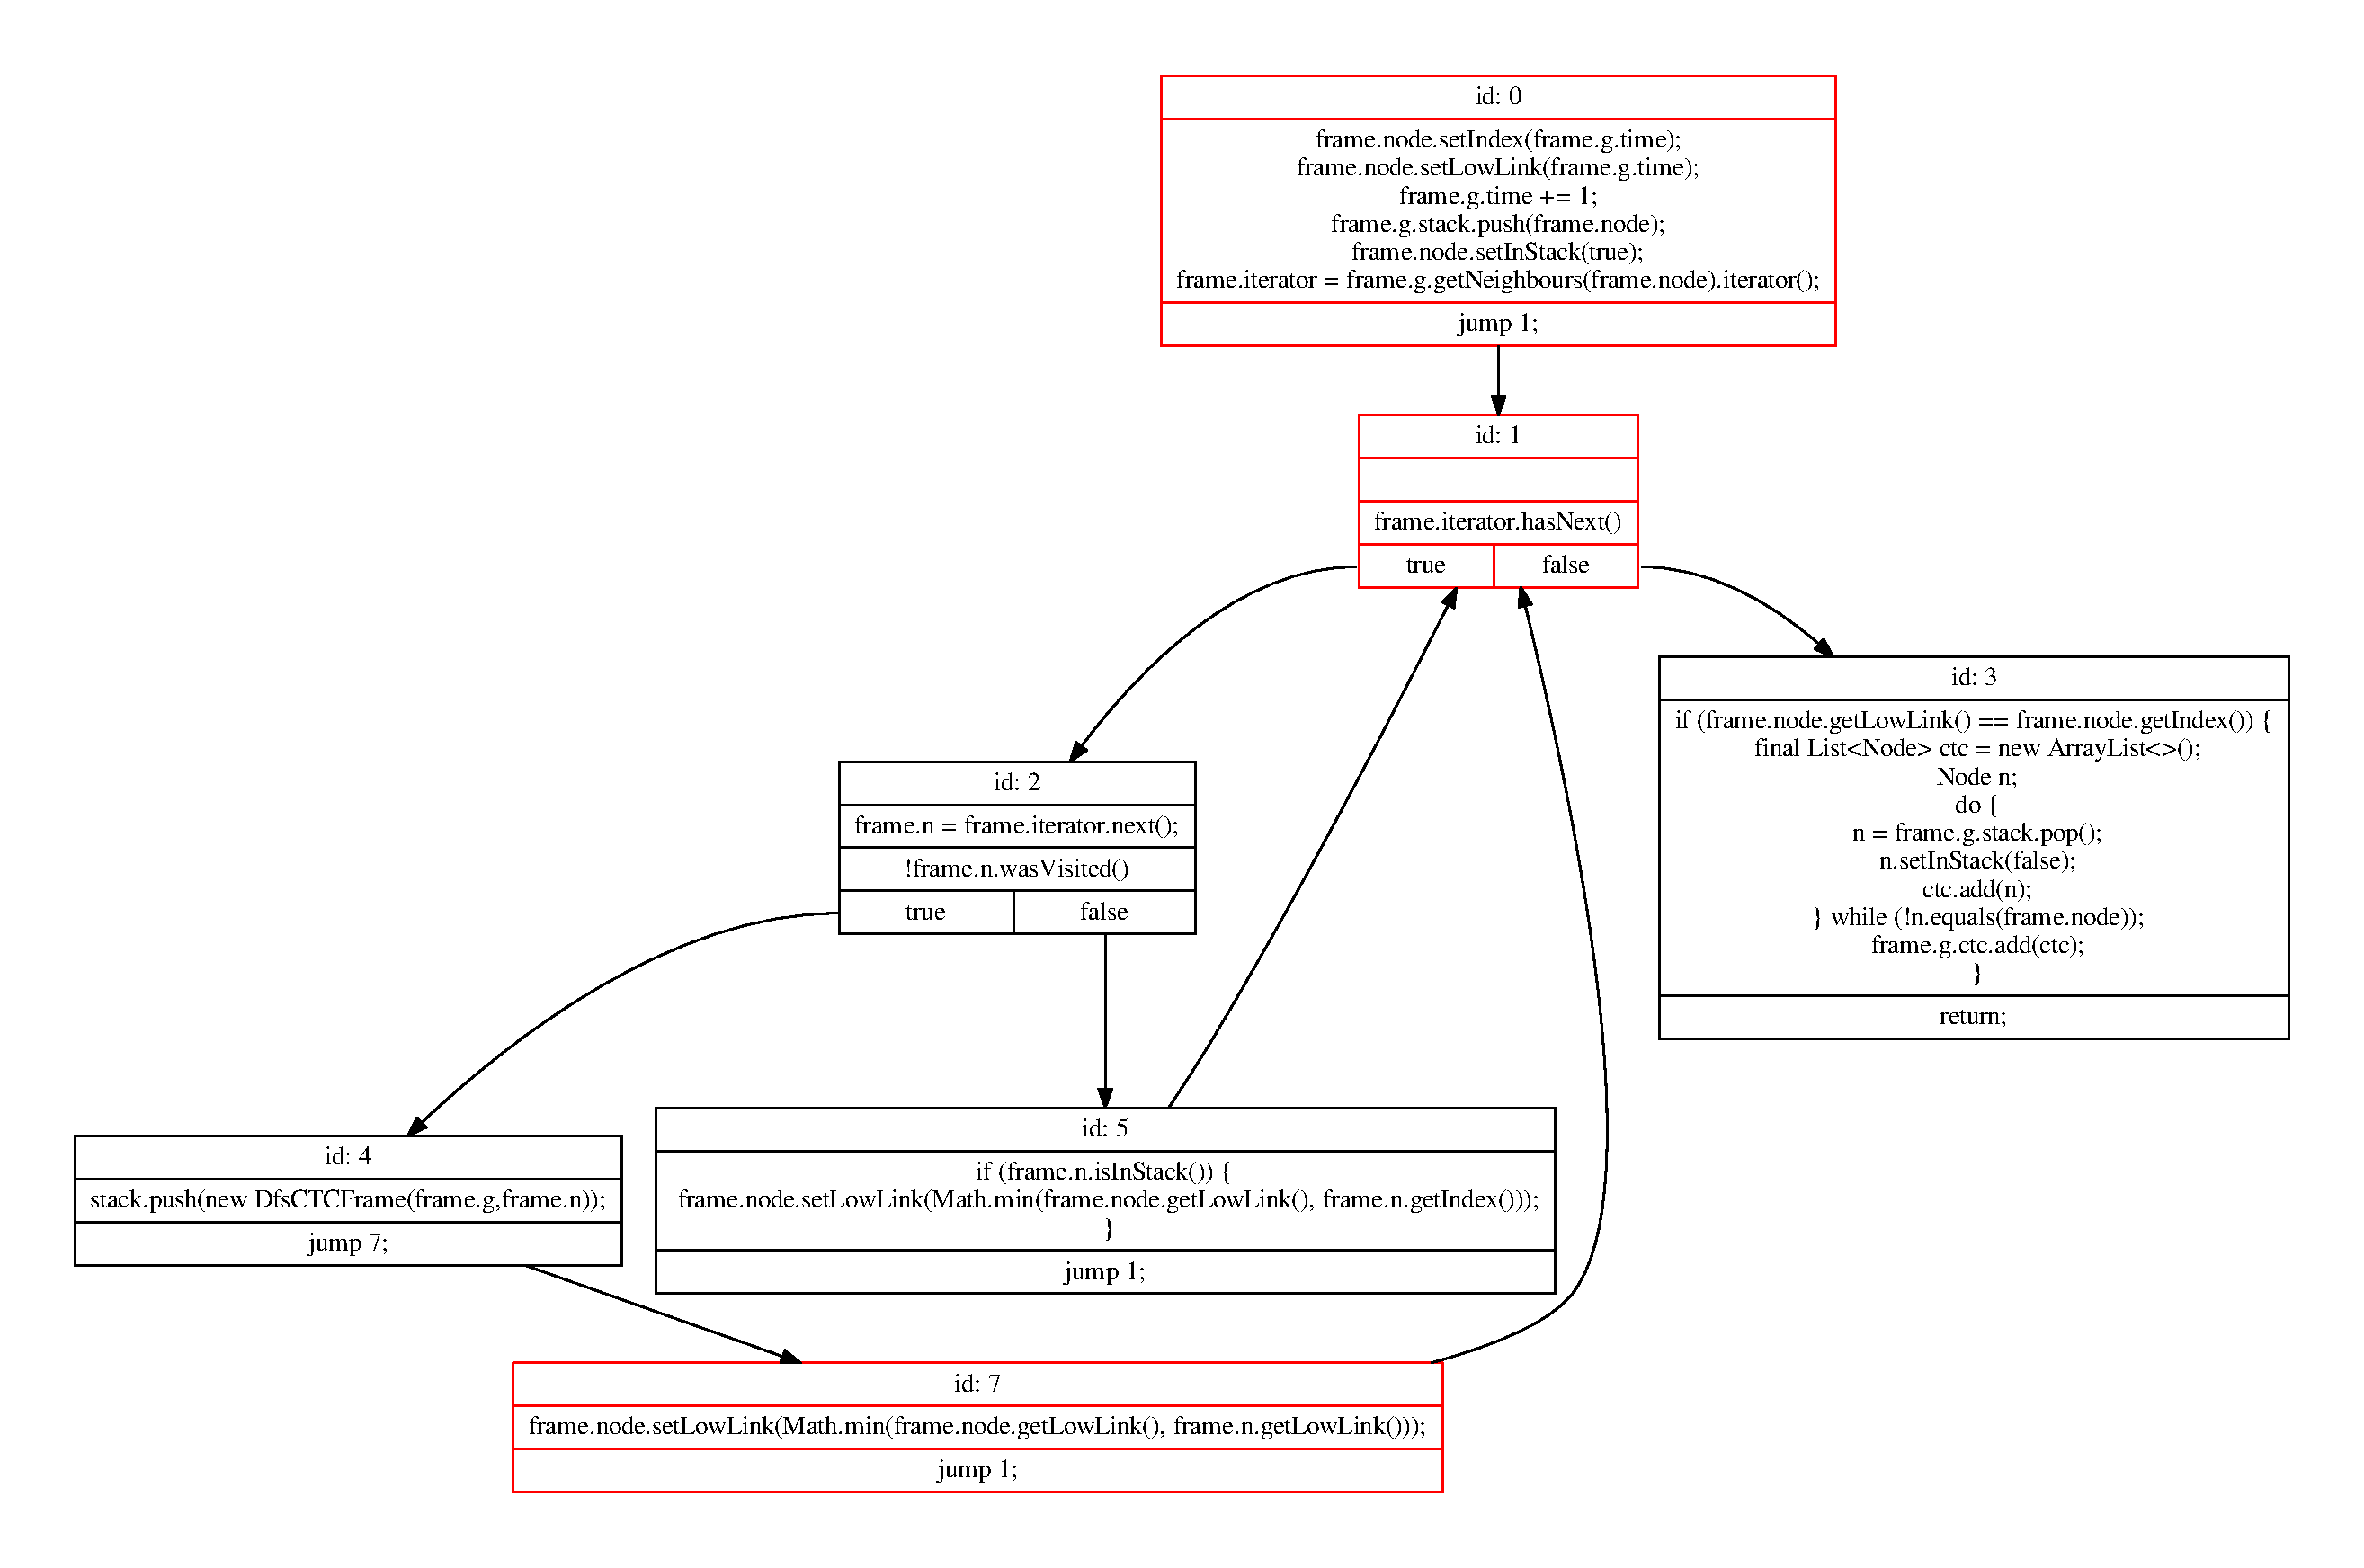
\includegraphics[width=\linewidth]{../../../theses/diploma/src/graph/trivial-after.pdf}
    \end{figure}
\end{frame}

%\begin{frame}{Reducerea grafului de control (Exemplu 1)}
%    \begin{figure}[htb]
%        \centering
%        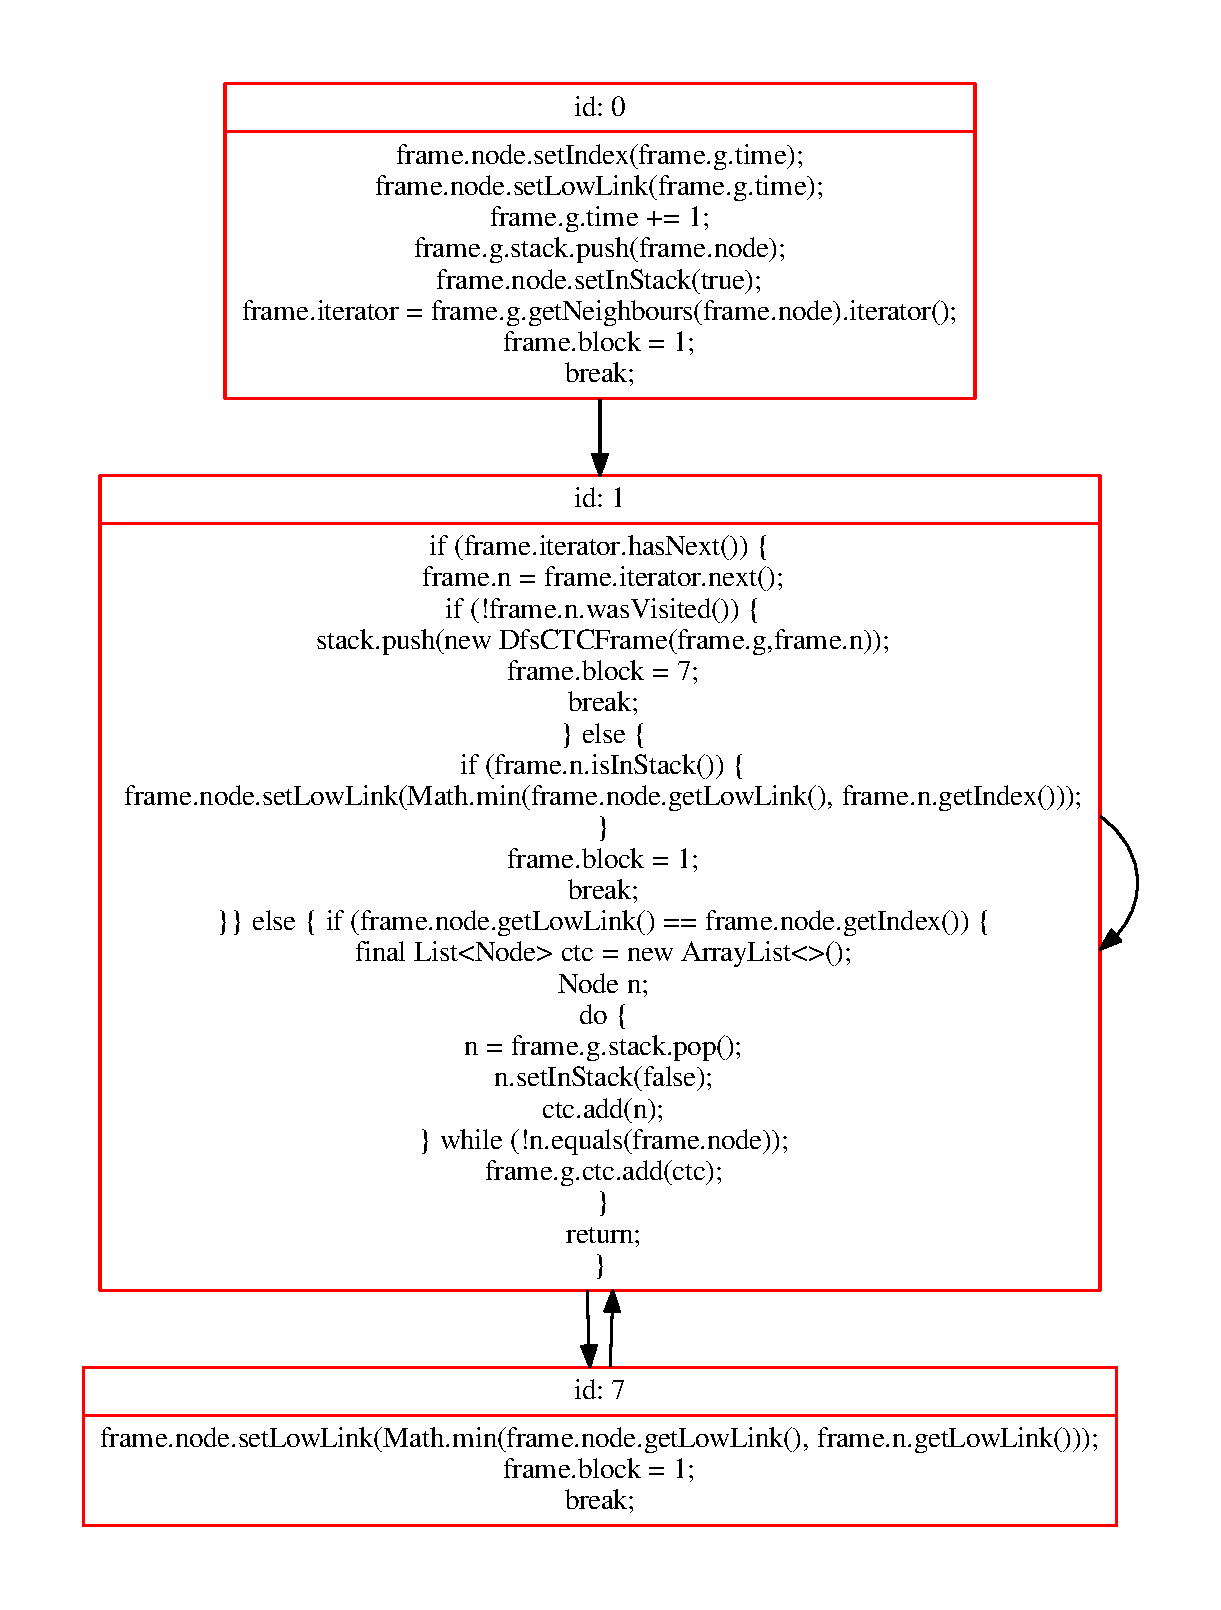
\includegraphics[width=.5\textwidth]{../../../theses/diploma/src/graph/inline-after-1.pdf}
%        \caption{The reduced CFG\label{img:inline1}}
%    \end{figure}
%\end{frame}

\begin{frame}{Reducerea grafului de control (Exemplu)}
% las doar exemplul mai mic
    \begin{figure}[htb]
        \begin{subfigure}[b]{.42\textwidth}
            \centering
            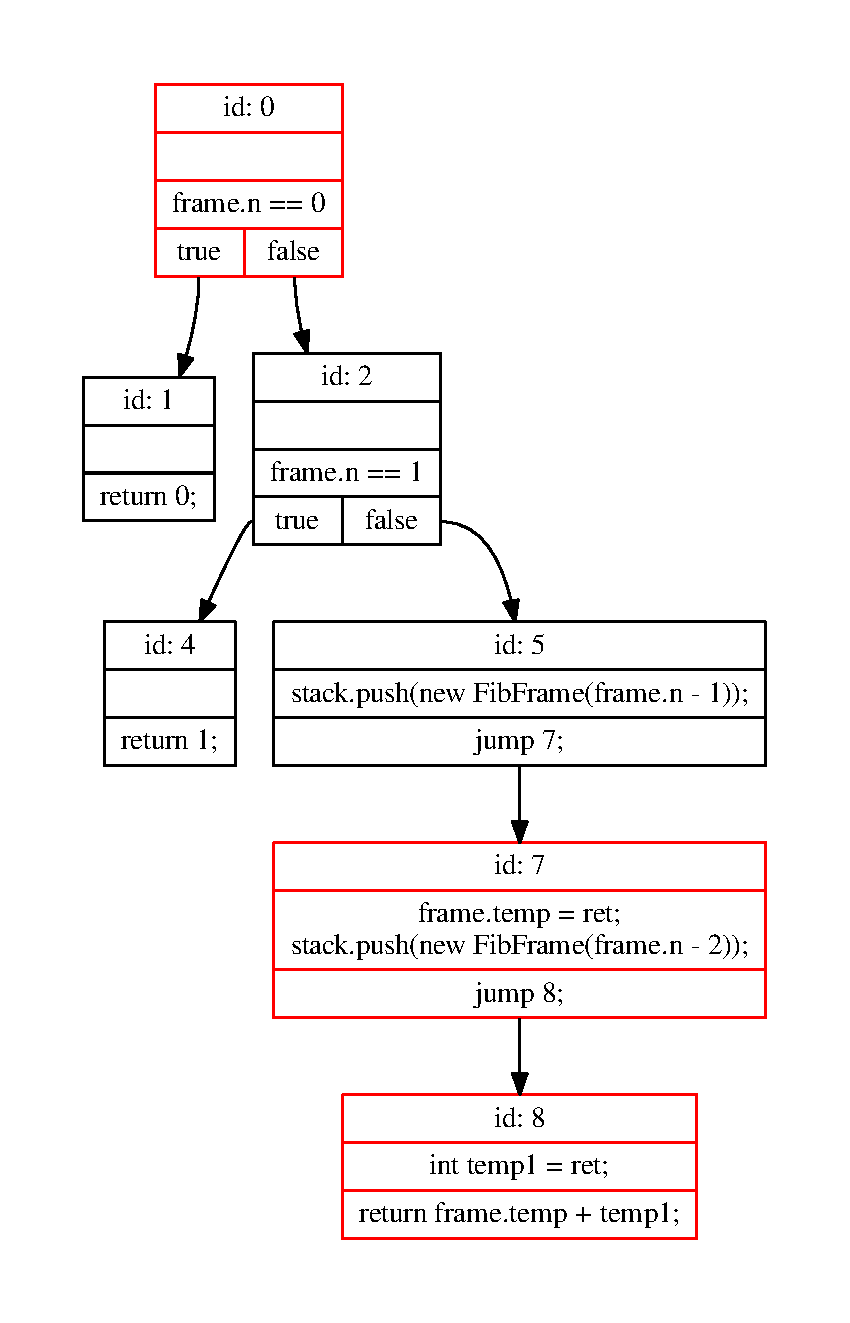
\includegraphics[width=\textwidth]{../../../theses/diploma/src/graph/inline-before.pdf}
            \caption{Înainte}
        \end{subfigure}
        \hfill
        \begin{subfigure}[b]{.42\textwidth}
            \centering
            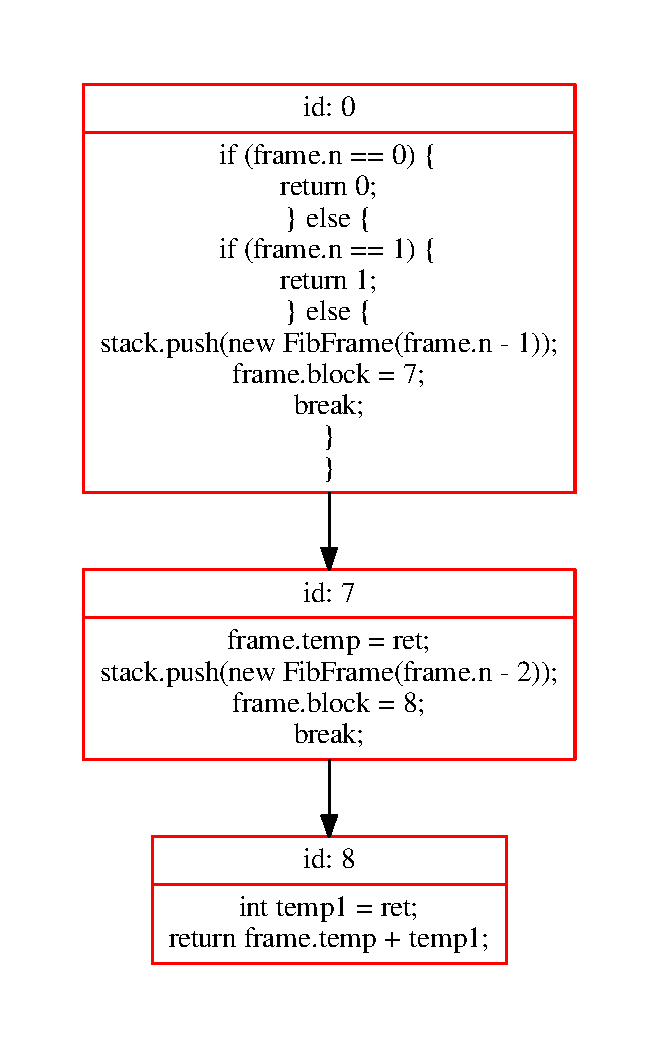
\includegraphics[width=\textwidth]{../../../theses/diploma/src/graph/inline-after.pdf}
            \caption{După}
        \end{subfigure}
    \end{figure}
\end{frame}

\begin{frame}{Înlocuirea instrucțiunii \code{return}}
    \begin{itemize}
        \item Atribuirea expresiei instrucțiunii \code{return} la variabila \code{ret}
        \item Eliminarea de pe stivă a înregistrării de activare curente
        \item Adăugarea unei instrucțiuni \code{break}
\end{itemize}
%    \begin{figure}[htb]
%        \begin{subfigure}[b]{.45\textwidth}
%            \centering
%            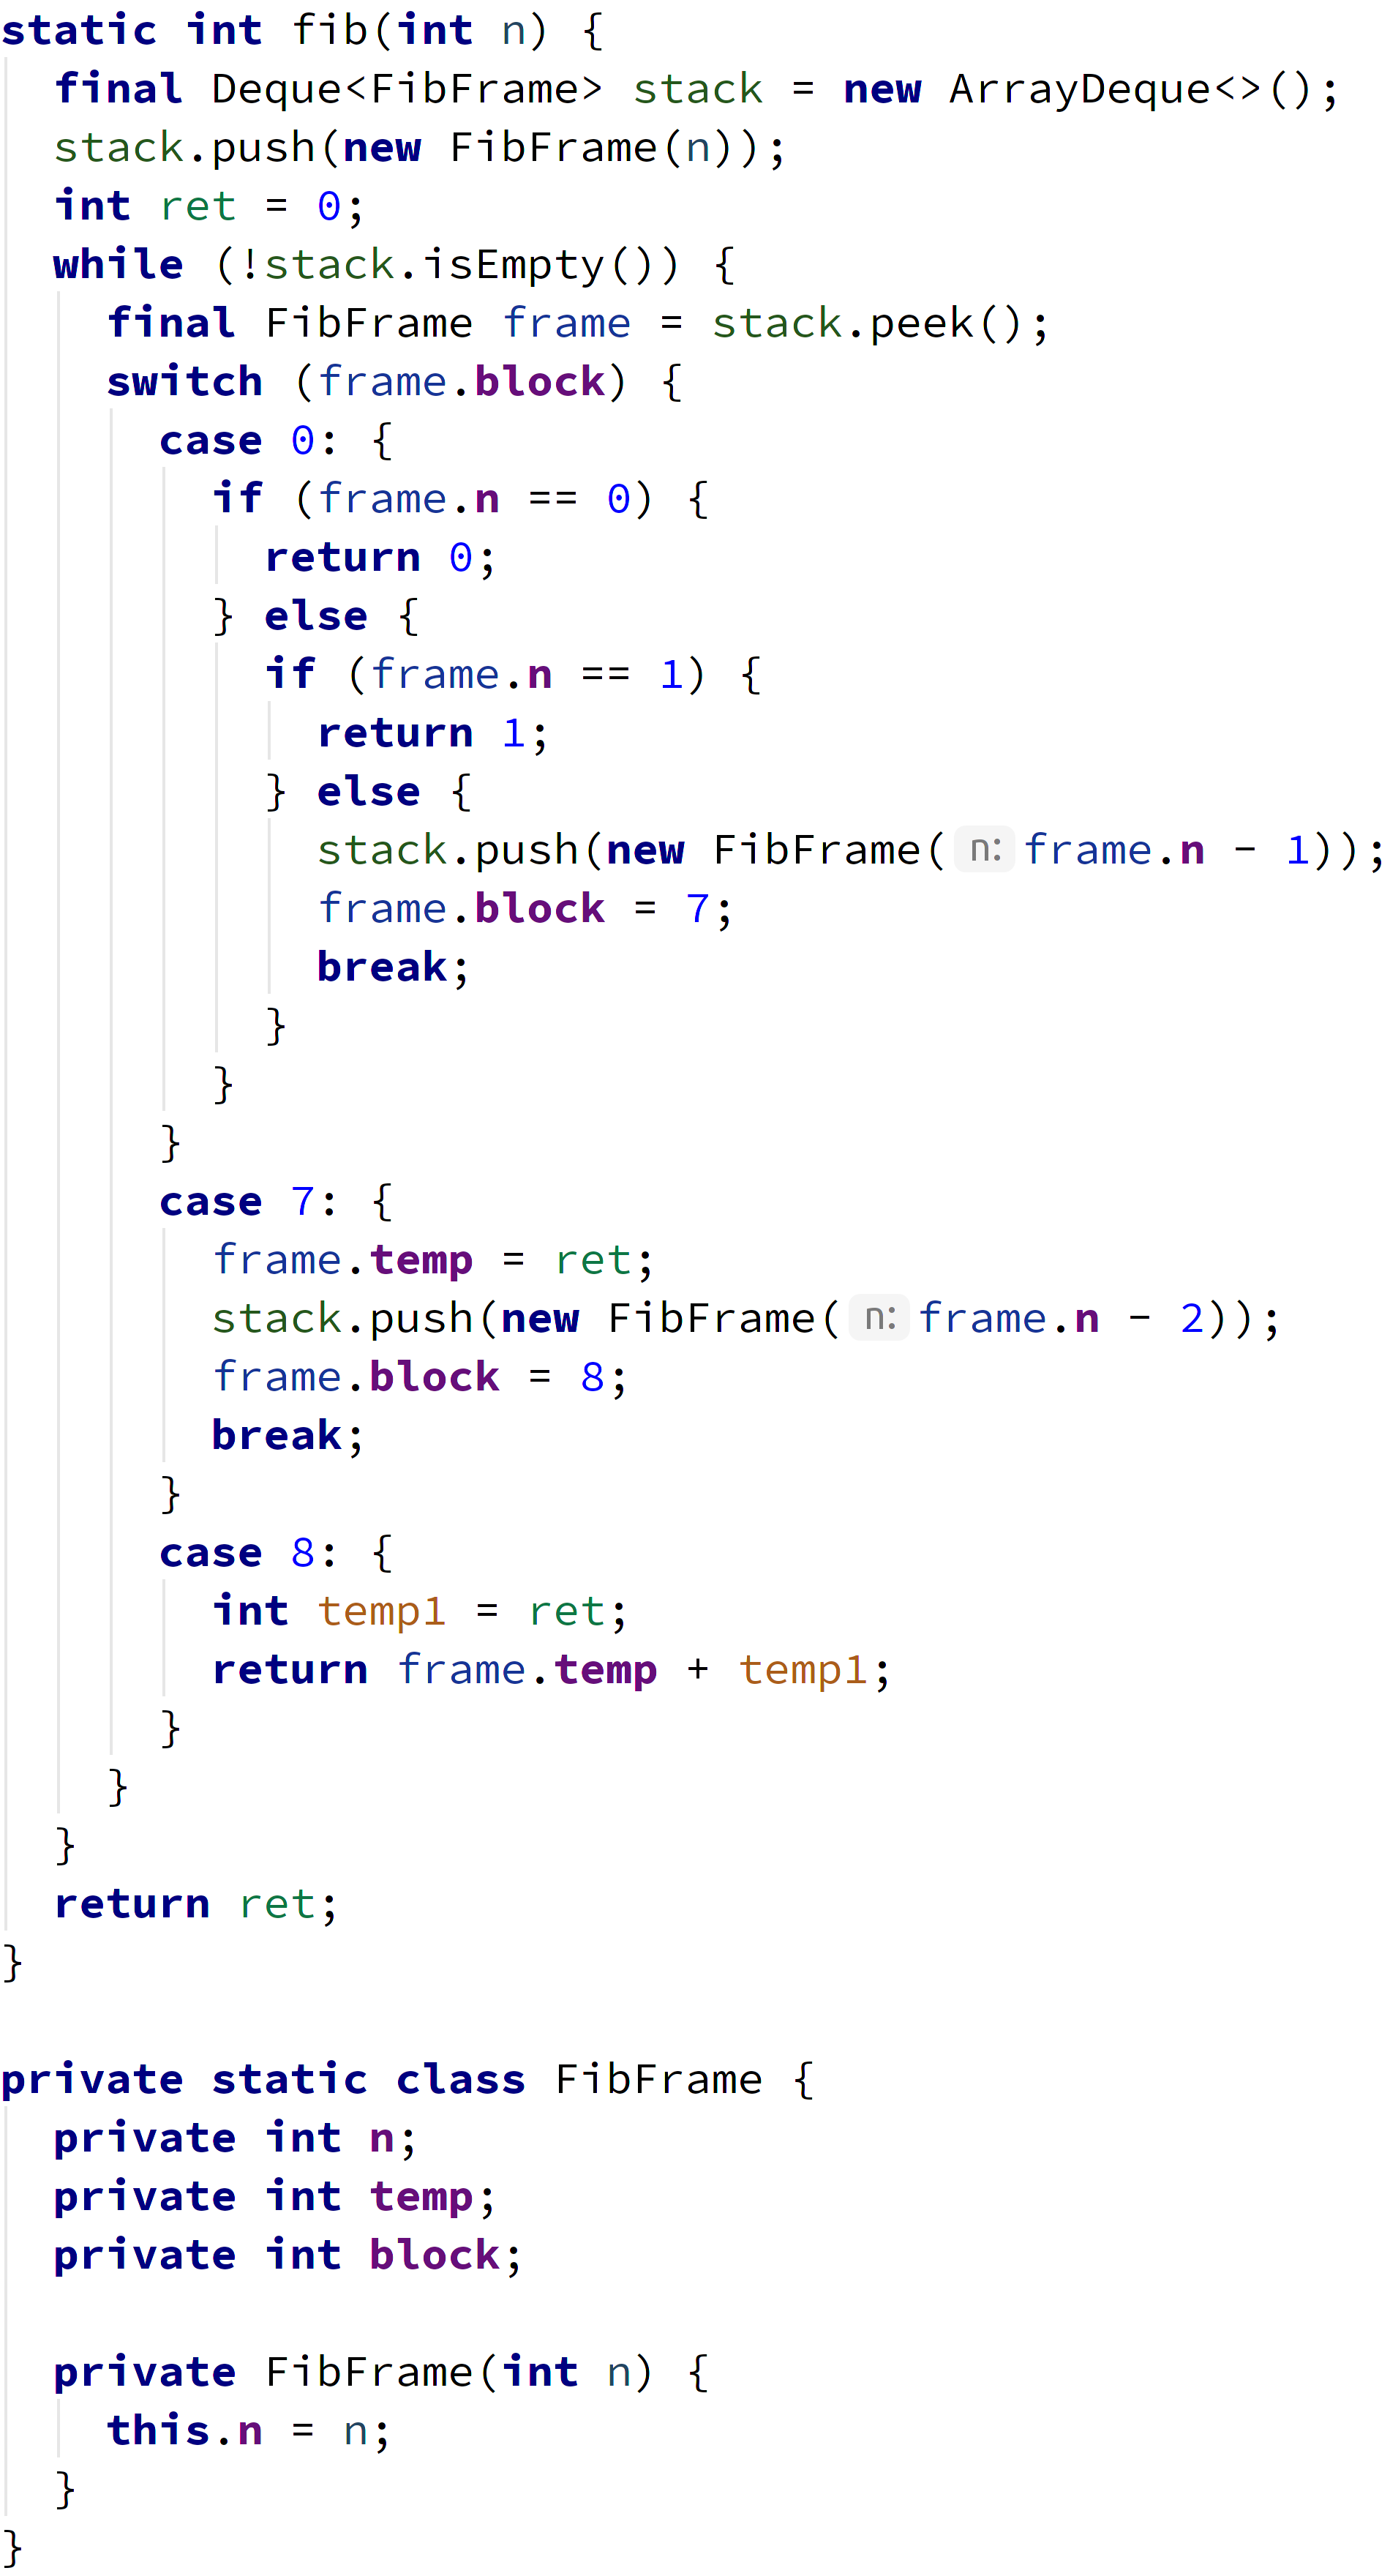
\includegraphics[height=2.3in]{../../../theses/diploma/src/img/inline-blocks-after-white-44.png}
%        \end{subfigure}
%        \begin{subfigure}[b]{.45\textwidth}
%            \centering
%            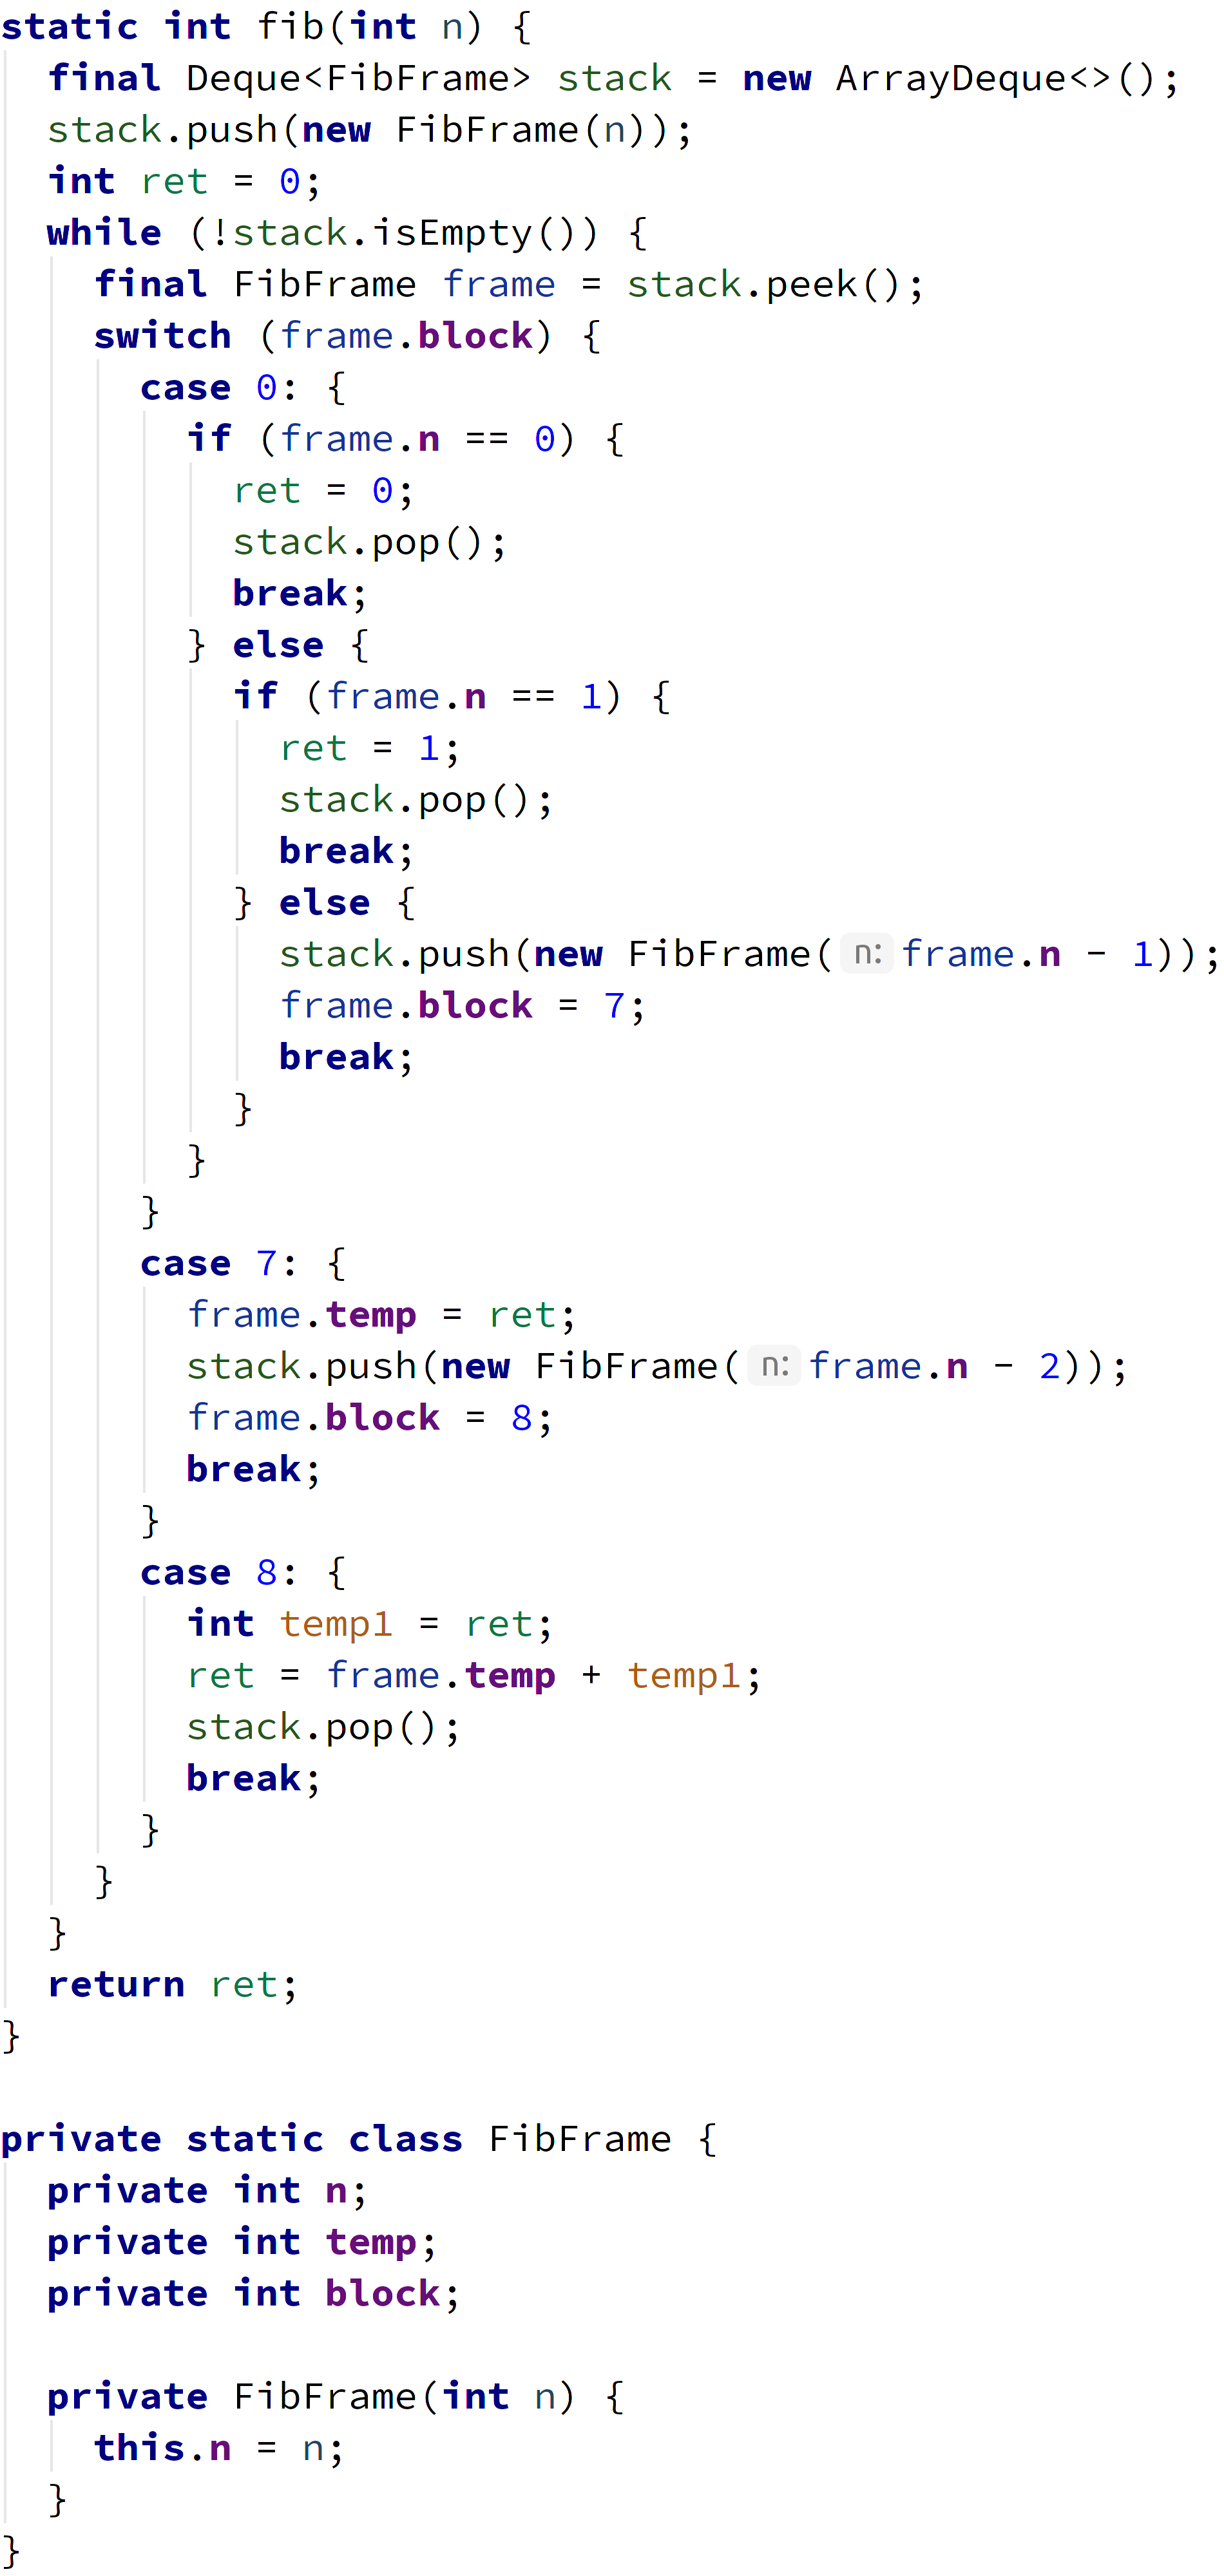
\includegraphics[height=2.617in]{../../../theses/diploma/src/img/replace-return-after-50.png}
%        \end{subfigure}
%    \end{figure}
\end{frame}

\section{Testare}

\begin{frame}{Testare}
    \begin{itemize}
        \item Validarea transformării corecte a codului prin teste unitare:
        \begin{itemize}
            \item Pentru fiecare etapă a algoritmului
            \item Pentru întreg algoritmul
        \end{itemize}
        \item Validarea conservării semanticii codului
    \end{itemize}
\end{frame}
	
\section{Evaluarea perfomanțelor}

\begin{frame}{Evaluarea performanțelor}
    \begin{itemize}
        \item Suma primelor 2000000 de numere prime
        \begin{itemize}
            \item Varianta recursivă: \code{StackOverflowError}
            \item Varianta iterativă: 2 secunde
        \end{itemize}
        \item Suma primelor 10000 de numere prime
        \begin{itemize}
            \item Varianta recursivă: 2ms
            \item Varianta iterativă: 6ms
        \end{itemize}
    \end{itemize}
%    \begin{figure}[htb]
%        \begin{subfigure}[b]{.45\textwidth}
%            \centering
%            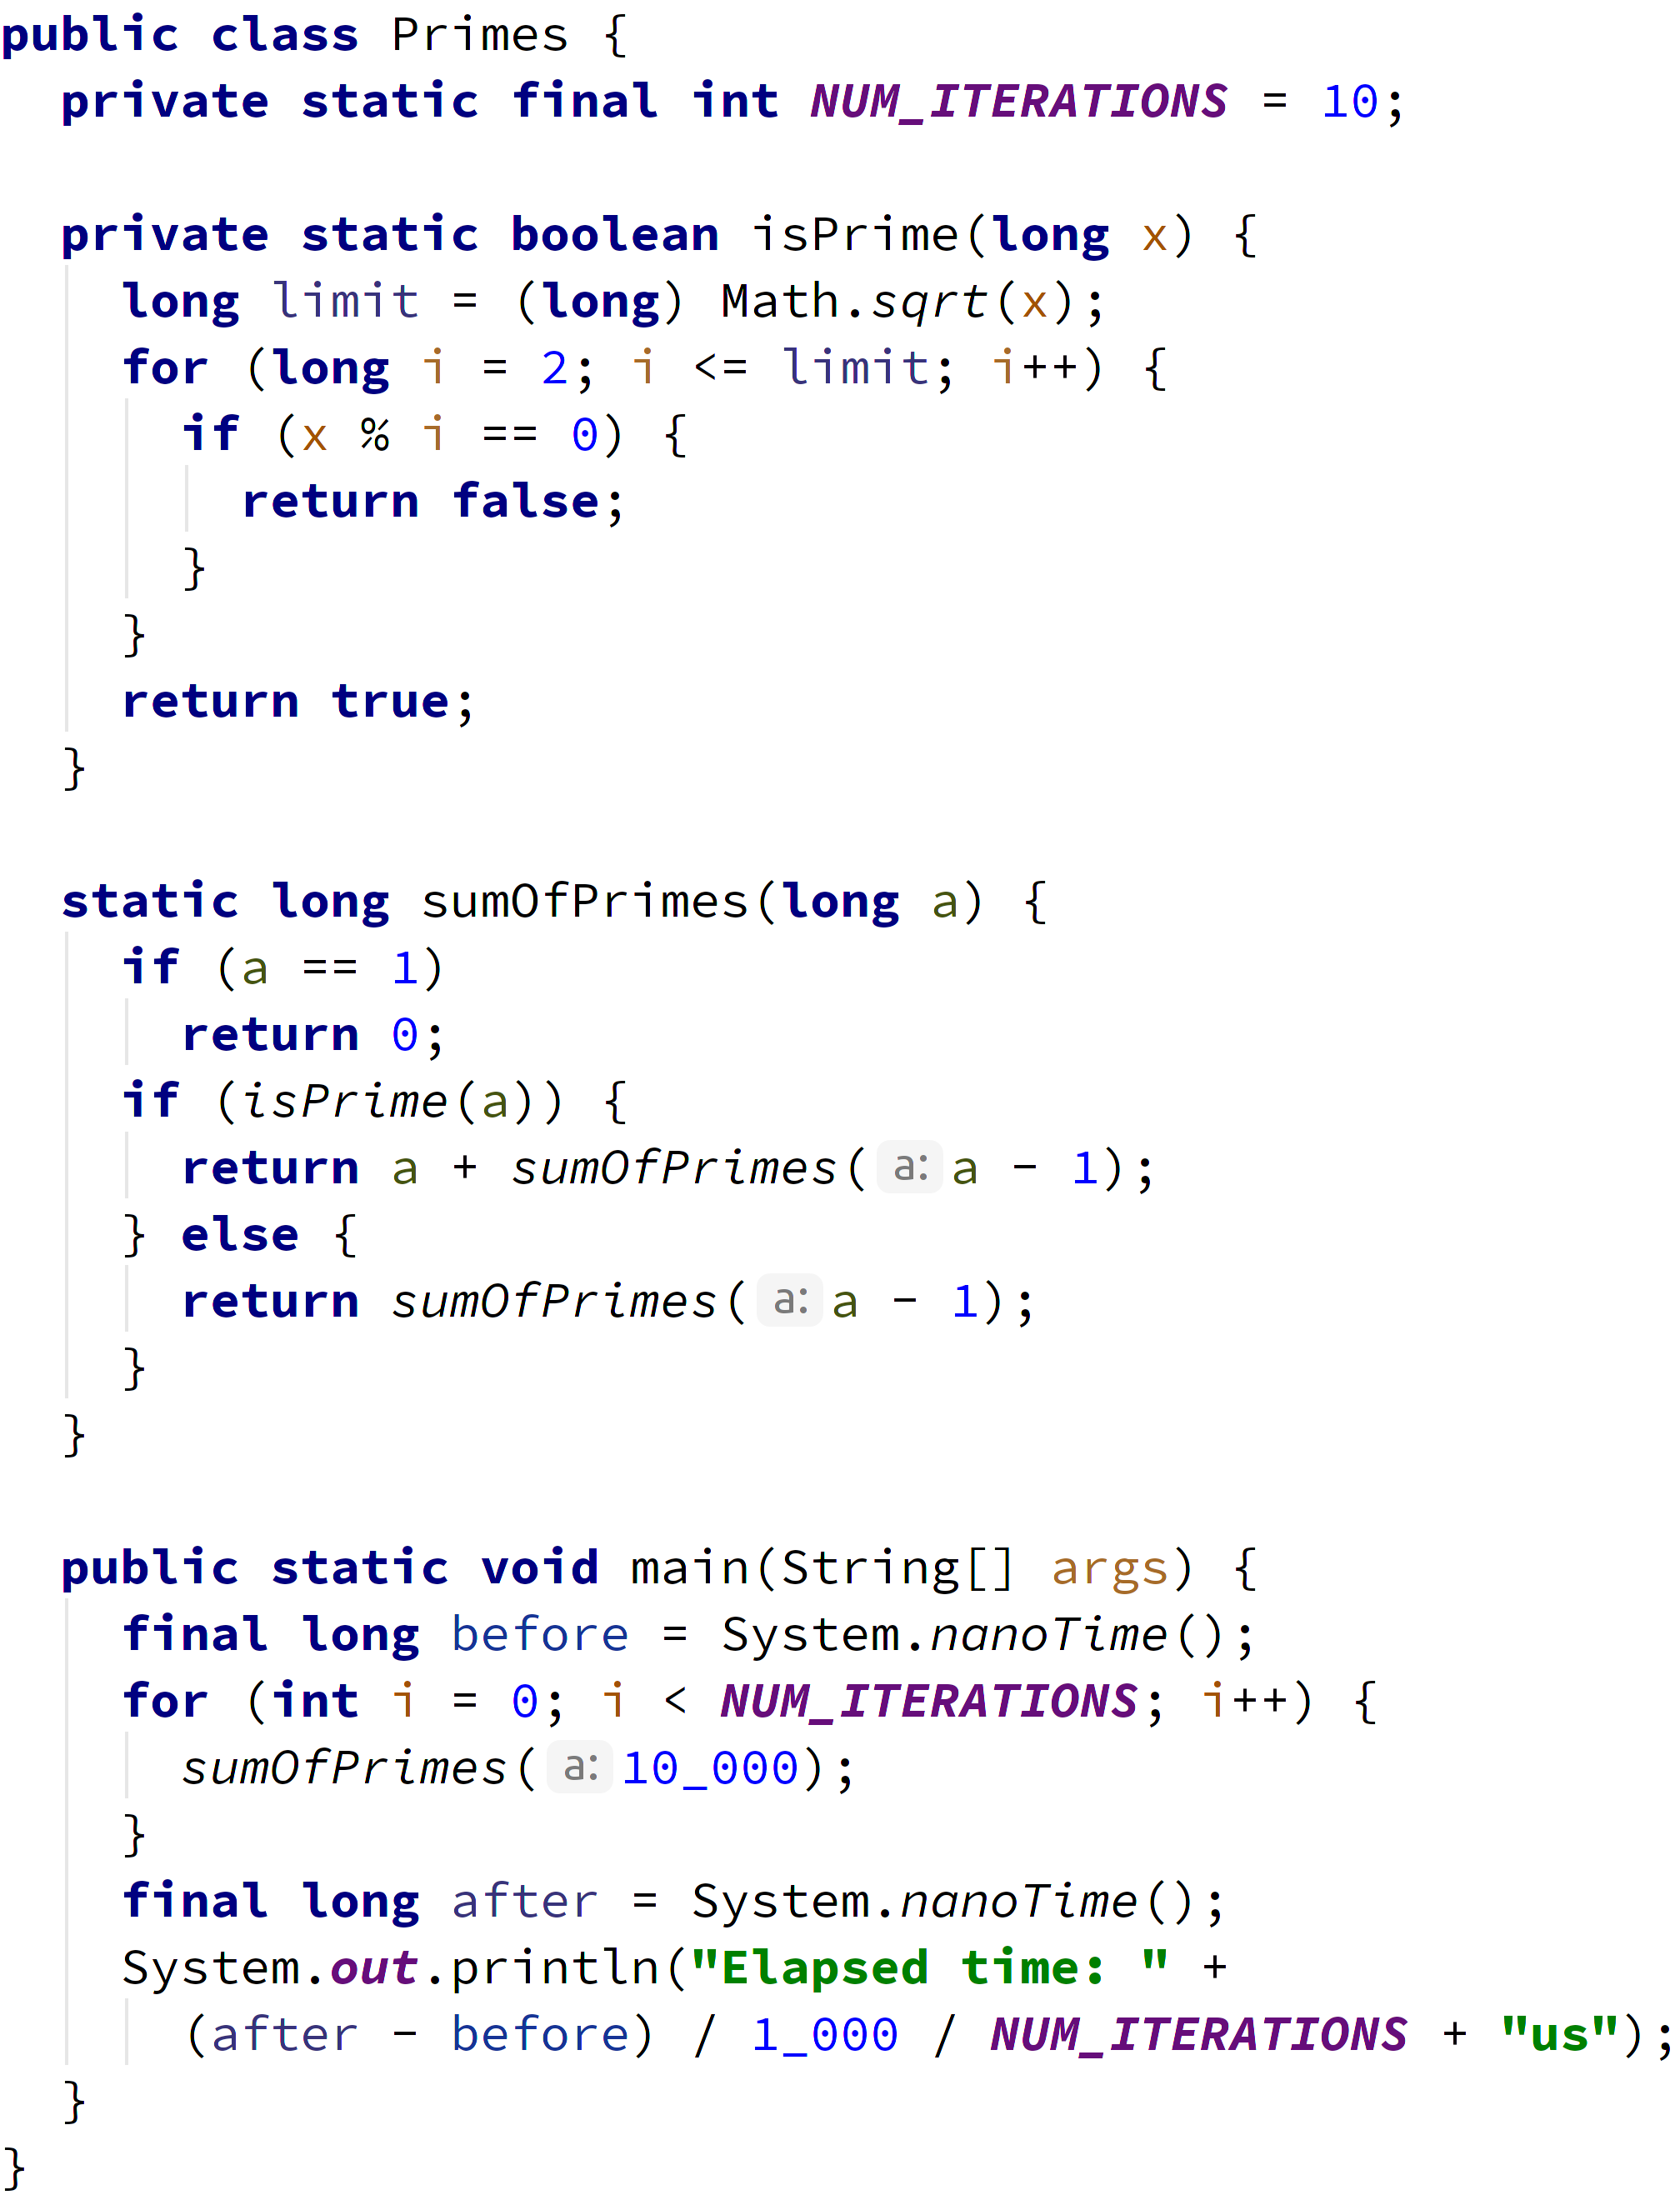
\includegraphics[height=2in]{../../../theses/diploma/src/img/primes-before-33.png}
%            \caption{2ms}
%        \end{subfigure}
%        \begin{subfigure}[b]{.45\textwidth}
%            \centering
%            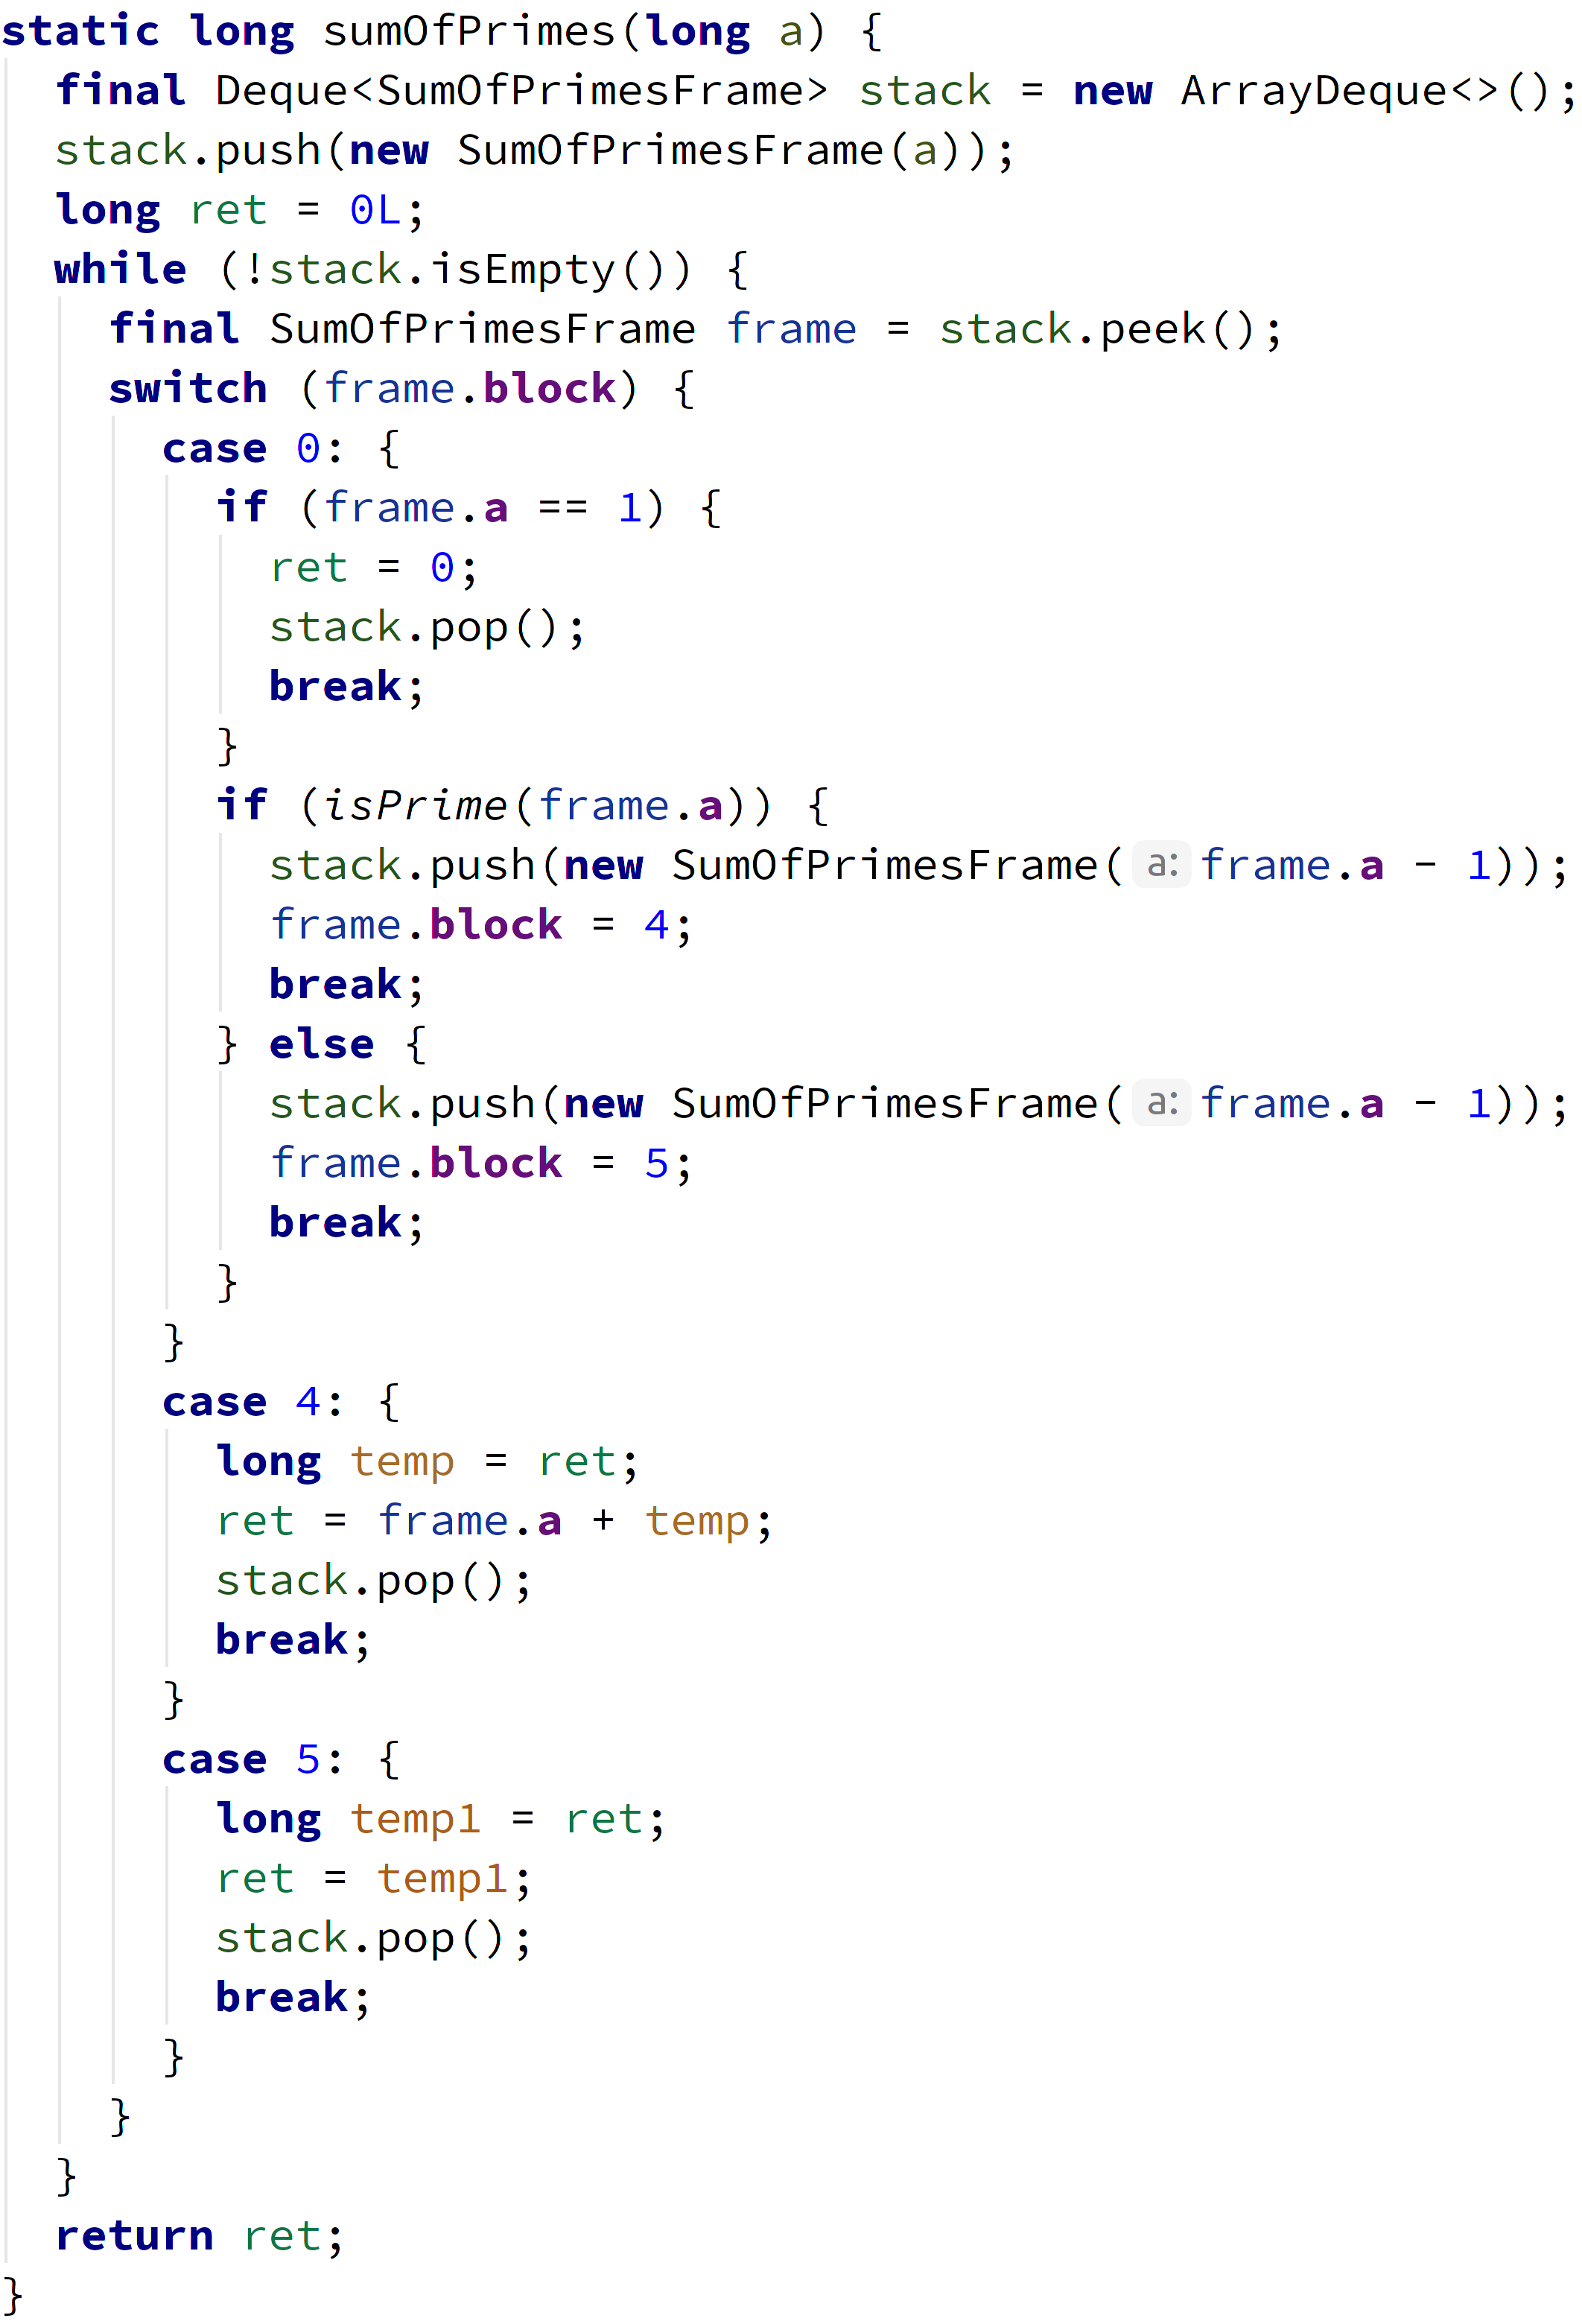
\includegraphics[height=2.36in]{../../../theses/diploma/src/img/primes-after-39.png}
%            \caption{6ms}
%        \end{subfigure}
%    \end{figure}
\end{frame}

%\begin{frame}{Suma primelor 2000000 de numere prime}
%    \begin{itemize}
%        \item Varianta recursivă: \code{StackOverflowError}
%        \item Varianta iterativă: 2 secunde
%    \end{itemize}
%\end{frame}

\section{Concluzii}

\begin{frame}{Concluzii}
    \begin{itemize}
        \item Rezolvă problema \code{StackoverflowError}
        \item Instrument ușor de folosit, integrat într-un mediu de dezvoltare
        \item Lizibilitatea codului poate fi afectată
    \end{itemize}
\end{frame}

\begin{frame}{Dezvoltări ulterioare}
	\begin{itemize}
        \item Optimizarea algoritmului de eliminare a recursivității
		\item Tratarea recursivității pe revenire
        \item Tratarea unor cazuri particulare de recursivitate pe avans
	\end{itemize}
\end{frame}

\end{document}
